\documentclass[12pt,oneside,letterpaper,article]{memoir}
\usepackage{indentfirst}                                    % All subsections indented
\usepackage{setspace}                                       % For 1.5 spacing
\usepackage{hyperref}                                       % Make table of contents clickable, allow URLs
\usepackage[letterpaper, margin=1in]{geometry}              % 1 inch margin, letter paper (American)
\usepackage[english]{babel}                                 % For "fancy" quotes
\usepackage[autostyle, english=american]{csquotes}          % Same
\usepackage{etoolbox}                                       % Misc
\usepackage{titlesec}                                       % Modify spacing
\MakeOuterQuote{"}                                          % For fancy quotes
\usepackage{times}                                          % For tilde
\usepackage{textcomp}                                       % For tilde
\usepackage{graphicx}                                       % Images
\usepackage{array}                                          % Table spacing
\usepackage{ragged2e}                                       % Left align table text
\usepackage{caption}                                        % Use to create the \repeatcaption command
\usepackage{float}                                          % Image placement
\usepackage[fit]{truncate}                                  % Truncate section names
\usepackage{charter}                                        % Charter font
\usepackage[acronym]{glossaries}                            % Glossary, acronyms list, etc
\usepackage{glossary-mcols}                                 % Multi-column glossary or acronyms list
\usepackage{xparse}                                         % Better parsing for macros
\usepackage[detect-all]{siunitx}                                        % SI unit formatting
\usepackage{appendix}                                       % Appendices
\usepackage{minted}                                         % Code!
\usepackage{amsmath}                                        % Math
\usepackage{caption}                                        % Captions for formulas

\hypersetup{colorlinks=true,                                % Blue hyperlinks, everything else black
            urlcolor=blue,
            citecolor=black,
            linkcolor=black}
\renewcommand\familydefault{\sfdefault}                     % Sans serif
\newcommand{\textapprox}{\raisebox{0.1ex}{\texttildelow}}   % Add a ~ character for approximate values
\newcommand{\repeatcaption}[2]{                             % \repeatcaption command for reusing figures
  \renewcommand{\thefigure}{\ref{#1}}
  \captionsetup{list=no}
  \caption{#2 (repeated from page \pageref{#1})}
}

% 1in margins
\setulmarginsandblock{1in}{1in}{*}
\setlrmarginsandblock{1in}{1in}{*}

% Sectioning whitespace
\setbeforesecskip{0.35em}
\setaftersecskip{0.2em}
\setlength{\beforesubsecskip}{0.2em}
\setlength{\aftersubsecskip}{.1em}
\setlength{\beforechapskip}{0.5em}
\setlength{\afterchapskip}{0.3em}
\setlength{\belowcaptionskip}{-0.1em}

% Show subsection numbers and entries in TOC
\setsecnumdepth{subsection}
\maxtocdepth{subsection}

% Macro for acronyms with description
\let\newacronymsaved\newacronym
% \def\?#1{}
\RenewDocumentCommand\newacronym{mmmg}{
    % Fuck all ye who enter here
    \expandafter\newcommand\expandafter{\csname #1\endcsname}[0]{\gls{#1}\,\,}
    \expandafter\newcommand\expandafter{\csname #1s\endcsname}[0]{\glspl{#1}\,\,}
    \expandafter\newcommand\expandafter{\csname #2\endcsname}[0]{\Gls{#1}\,\,}
    \expandafter\newcommand\expandafter{\csname #2s\endcsname}[0]{\Glspl{#1}\,\,}
    \IfNoValueTF{#4}{
        \newacronymsaved{#1}{#2}{#3}
    } {
        \newglossaryentry{#1}{
                            type=\acronymtype, 
                            name={#2}, 
                            description={#3}, 
                            first={#3 (#2)\glsadd{#1-gls}}, 
                            plural={⟨#2⟩\glspluralsuffix},
                            firstplural={⟨#3⟩\glspluralsuffix\space (⟨#2⟩\glspluralsuffix)},
                            see=[Glossary:]{#1-gls}}
        \newglossaryentry{#1-gls}{name={#2}, description={#4. \textit{See pgs}}}
    }
}

% Some new units
\DeclareSIUnit{\dollar}{\$}
\DeclareSIUnit{\bit}{b}
\DeclareSIUnit{\byte}{B}

% Captioned equation (formula) environment
\DeclareCaptionType{formula}[][]
\captionsetup[formula]{name=Formula,labelformat=default,font={it,small},margin=0.5in}
 % Don't question it
\usepackage{styles/listofauthorships}
\usepackage{multicol}
\usepackage[style=ieee,citestyle=numeric-comp,sorting=anyt]{biblatex}
\usepackage{wrapfig}
\usepackage{placeins}
\usepackage{microtype}
\usepackage{float}
\graphicspath{{images/}}

\title{\scshape Mapping Internet Connectivity in the United States}
\author{Samuel Goldman, Evan Goldstein, Christopher Myers, David Vollum}
% \date{September 2019}

% Glossary info goes in the preamble
\makeglossaries
% \todo{Fix numbering}
% Acronyms
% Follow the form: \newacronym{label}{ACRONYM}{expansion}
% Also: alphabetize!
\newacronym{api}{API}{application programming interface}
\newacronym{aws}{AWS}{Amazon Web Services}
\newacronym{caida}{CAIDA}{Center for Applied Internet Data Analysis}
\newacronym{cdf}{CDF}{cumulative distribution function}
\newacronym{cli}{CLI}{command-line interface}
\newacronym{cors}{CORS}{cross-origin resource sharing}
\newacronym{csv}{CSV}{comma separated value}
\newacronym{ddos}{DDoS}{distributed denial of service}
\newacronym{dns}{DNS}{domain name system}
\newacronym{dsl}{DSL}{digital subscriber line}
\newacronym{fcc}{FCC}{Federal Communications Commission}
\newacronym{gdp}{GDP}{gross domestic product}
\newacronym{gis}{GIS}{geographic information system}
\newacronym{gps}{GPS}{global positioning system}
\newacronym{html}{HTML}{Hypertext Markup Language}
\newacronym{http}{HTTP}{hypertext transfer protocol}
\newacronym{httpse}{HTTPS}{hypertext transfer protocol secure}
\newacronym{idw}{IDW}{inverse distance weighting}
\newacronym{iqr}{IQR}{inter-quartile range}
\newacronym{ip}{IP}{internet protocol}
\newacronym{ipaoc}{IPoAC}{internet protocol over avian carrier}
\newacronym{ipvs}{IPv6}{internet protocol version 6}
\newacronym{ipvf}{IPv4}{internet protocol version 4}
\newacronym{json}{JSON}{Javascript Object Notation}
\newacronym{jwt}{JWT}{\json Web Token}
\newacronym{mbps}{Mbps}{megabits per second}
\newacronym{mqp}{MQP}{major qualifying project}
\newacronym{ntp}{NTP}{Network Time Protocol}
\newacronym{ripe}{RIPE}{R\'eseaux IP Europ\'eens}
\newacronym{rtt}{RTT}{round trip time}
\newacronym{sdk}{SDK}{software development kit}
\newacronym{svg}{SVG}{scalable vector graphics}
\newacronym{tcp}{TCP}{transmission control protocol}
\newacronym{tld}{TLD}{top level domain}
\newacronym{tls}{TLS}{transport layer security}
\newacronym{ttl}{TTL}{time-to-live}
\newacronym{acUrl}{URL}{uniform resource locator}
\newacronym{us}{US}{United States}
\newacronym{usps}{USPS}{United States Postal Service}
\newacronym{voip}{VoIP}{voice over internet protocol}
\newacronym{wpi}{WPI}{Worcester Polytechnic Institute}

% Acronyms with definitions
% Follow the form: \newacronym{label}{ACRONYM}{expansion}{description}. Description appears in glossary only.
\newacronym{anova}{ANOVA}{analysis of variance}{Analysis of variance is a class of statistical models and methods for estimation, used to analyze the difference between the means of a sample. Although there are many types, they all fundamentally calculate the probability (a $p$ value) that two population means are equal}

\newacronym{cdn}{CDN}{content delivery network}{A content distribution network, sometimes called a Content Delivery Network, is a network of proxy servers that form a kind of cache used to enhance delivery of content to internet users. Although helpful for internet users, they complicate measurements of connectivity to websites \textit{actually} connecting to the site's servers}
 
\newacronym{cv}{CV}{coefficient of variation}{Coefficients of variation, or relative standard deviations, are defined as the ratio of the absolute value of the mean of a variable divided by its standard deviation: $\frac{\lvert\mu\rvert}{\sigma}$. CVs are dimensionless values that can be judged independent of the original source, making them useful for gauging the spread of any data set. The lower the CV, the lower the spread of the data and the better the quality}
 
\newacronym{ecc}{EC2}{Amazon Elastic Compute Cloud}{EC2 is a service from Amazon Web Services that provides virtual machines in the cloud for general-purpose or task optimized work. EC2 can be configured for different performance and pricing classes, as well as complex auto-scaling schemes or virtual private cloud setups}
 
\newacronym{etl}{ETL}{extract-transform-load}{Extract-transform-load is a generic procedure for extracting data, transforming it into a more useful format, and loading it into a large volume storage system, such as a database. The term closer describes an architecture rather than a specific algorithm}
 
\newacronym{icmp}{ICMP}{internet control message protocol}{Internet Control Message Protocol is a protocol designed for error reporting and other utility purposes across the internet, typically used most by routers and other intermediary devices}

\newacronym{isp}{ISP}{internet service provider}{An internet service provider is typically the "last mile" organization that provides a user with internet access --- otherwise known as a \textit{tier 3} ISP. They are distinct from tier 2 and tier 1 ISPs which are responsible for much of the internet backbone, although ISP corporations may operate on multiple tiers. Common ISPs in the US include AT\&T, Comcast, and Verizon}
 
\newacronym{kde}{KDE}{kernel density estimation}{Kernel density estimation is a technique for estimating the probability density function of a variable. Briefly, KDEs work by processing each measurement of a variable as if it was at the center of some given probability density function, e.g. a gaussian curve. These curves are then summed together to form one curve and normalized so the area underneath the curve is equal to 1. A KDE chart can be read in the same way as a histogram can, but the $y$ axis corresponds to a density instead of an absolute value. The advantage to using a KDE over a histogram is that KDEs are not vulnerable to binning effects (from choosing the wrong bin size) while histograms are}

% Glossary entries -- these should be more detailed.
% Follow the form: \newglossaryentry{LABEL}{name={NAME} description={YOUR TEXT HERE}}
% \newglossaryentry{favicon}{
%     name={favicon},
%     description={Favicons are small identifying images, typically logos or relevant UI elements, that most websites provide for browsers to place on tabs and bookmarks. Favicons are stored as .ico files (icons) and are either 16x16, 32x32, or 48x48. This small size makes them ideal for testing connection \rtt from a browser}
% }

% \newglossaryentry{backbone}{
%     name={internet backbone},
%     description={Internet backbone infrastructure consists of high speed principal data routes and the connected major computer networks and core routers. For any trip of serious distance (likely most connections, unless you happen to have a data center in your backyard), packets will inevitably pass through some element of the internet backbone}
% }

% \newglossaryentry{traceroute}{
%     name={traceroute},
%     description={A traceroute is a technique that shows the full path data takes to get from your computer to a remote server, and how long it takes to get to each server along the way. Traceroutes leverage \icmp and specifically-set \ttl values to inciteintermediate servers to respond with an \icmp packet indicating the data packet's \ttl has expired -- thereby giving away the server's presence along the route}
% }


% Bibliography goes in the preamble
\bibliography{references}


\begin{document}
    %%%%%%%%%%%%%%%%%%%%
    %%% FRONT MATTER %%%
    %%%%%%%%%%%%%%%%%%%%
    
    % Title page
    % TODO MAKE A FANCY TITLE PAGE
    \pagenumbering{gobble}
    \maketitle
    \newpage
    
    % Abstract
    \begin{abstract}
We evaluated internet connectivity in the United States, drawn from different definitions of connectivity and different methods of analysis. Using DNS cache manipulation, traceroutes, and a crowdsourced “web ping” method we identify patterns in connectivity that correspond to higher population or coastal regions of the US. We analyze the data for quality strengths and shortcomings, establish connectivity heatmaps, state rankings, and statistical measures of the data. We give comparative analyses of the three methods and present suggestions for future work building off this report.
\end{abstract}
    \newpage
    
    % Table of contents, list of figures
    \pagenumbering{roman}
    \tableofcontents\newpage
    % \listofauthorships
    \listoffigures
    \listoftables
    \newpage
    
    % Switch to arabic page numbering, start headers, and one half spacing.
    \pagenumbering{arabic}
    \pagestyle{headings}
    
    %%%%%%%%%%%%%%%%%%%%%%%%%%%
    %%% MAIN PAPER CONTENTS %%%
    %%%%%%%%%%%%%%%%%%%%%%%%%%%
    
    % TO ADD SIGNIFICANT CONTENT:
    % Add a .tex file under the text folder, put your stuff there, then \input it in the
    % spot where it should go. THIS MEANS YOU DON'T HAVE TO DEAL WITH ONE GIANT MANUSCRIPT!
    
    \chapter{Introduction}\label{sec:introduction}
    Internet access is an increasingly important part of the American economy and everyday life. Functions as simple as applying for a job, keeping in touch with friends, or continuing self-education all require internet connectivity. Major technology firms are often in the public spotlight, and common internet services can be found everywhere in public, ranging from music and video streaming, to online e-book stores, to digital storefronts. For a more quantitative evaluation, in 2018 an industry group comprised of major technology firms estimated that the "internet sector" of the economy alone represented \$2.1 trillion a year, or about 10\% of the \us economy \cite{Shepardson2019InternetGroup}.

Unfortunately not all parts of the \us are as well connected as others, even by measures from simple personal anecdotes. For instance, it is  quite possible to find a town in rural Indiana where the best connection isn't good enough to stream a movie, while driving just 45 minutes east will yield a connection an order of magnitude better. Subjective measures and tales like this are common everywhere across the \us, but there is little scientifically-rigorous or complete data available. For instance, the \fcc has a map of estimated broadband deployment \cite{FederalCommunicationsCommission}, but simple broadband deployment isn't necessarily a good measure of how well connected people in those areas actually are.

To address these problems, we set out to gather and analyze as much data as we could on how well connected Americans are to the internet, using various means and measures. Our hypothesis is simple: although there may be some regional variations or "spottiness," there is a relationship between your location in the \us and what sort of internet service you can expect. We hypothesized that areas near each other are likely to have similar connectivity to one another, and that these similarities will form large scale trends that should be visible on a map, both visible and interpretable by non-technical readers.

The end goal of our project was to find if such relationships exist, and if so, to conduct analyses on the data to make the differences between areas of the \us clear. An important quality of our work is that it should be scientifically rigorous and statistically valid -- that is, we should avoid systemic error and account for random error in our calculations -- so a great deal of effort was expended on ensuring the validity of our results.

The reminder of the report is organized into chapters as follows:

In \cref{sec:background} we present background information on the fundamentals of the internet, information relevant to our methods, and research conducted on prior works and attempts at measuring connectivity.

In \cref{sec:connectivity_defs} we rely upon collected background research to define some metrics for internet connectivity. These are not limited to traditional metrics used by consumers (such as speed), instead taking a more expansive approach.

\Cref{sec:methods} describes a brief overview of our three main methods for collecting \& analyzing data on internet connectivity. We also present a brief overview of some of the statistical methods used, and an explanation of some methods that were considered but ultimately rejected.

\Crefrange{sec:caida}{sec:dns} present detailed methods of the design, implementation, and analysis for each of our three methods for collecting data. Their analyses differ since each dataset is somewhat different, but the fundamentals (e.g. definitions of connectivity) remain largely the same.

\Cref{sec:comparative_analyses} contains our comparative analysis of the results of the three data analyses. We present overall conclusions drawn from the data, in both things we assert we are confident of and things we assert we are uncertain of.

Finally, in \cref{sec:future_work} we suggest ideas for future projects to follow up on, drawing from shortcomings noted in our methods and the unpursued methods explained in \cref{sec:methods}.

\todo{Should we include the conclusion in the roadmap?}

    
    \newpage
    \chapter{Background}\label{sec:background}
    This chapter presents an overview of the of foundations the Internet and elements critical to understanding how our methods and analyses work. \Cref{sec:background_internet_architecture} covers the basics of how Internet the Internet is organized, while \cref{sec:speed_test_background} provides an example of a common metric that consumers use to test their Internet access and \cref{sec:background_traceroutes} explores how traceroutes can be used to analyze a network connection's path. \Cref{sec:background_caching} explains how various forms of caching, while \cref{sec:background_cdns} gives an overview of caching's close cousin, the \cdn. \Cref{sec:background_geolocation} presents an overview of the methods used to assign a location to an \ip address, which is critical to all parts of this report. Finally, \cref{sec:background_prior_work} details some past attempts to understand Internet connectivity in the \us.


    \section{Internet Connectivity}\label{sec:background_connectivity}
\textit{Assigned to: David}

To measure internet connectivity, it's important to concretely define \textit{what} internet connectivity is. To that end we've put together a list of possible metrics for defining internet connectivity.

\subsection{RTT to all other locations}[Chris M.]
\label{sec:raw-rtt-everything}

\RTT is a measure of how long it takes for a packet to reach a server plus the time it takes for the server's response to make it back to the original source. It has a major effect on the apparent latency of a connection or the quality of a streaming application such as video streaming, video calls, \voip calls, and multiplayer gaming. Lower \rtts indicate a better connection and a more responsive internet experience.

By measuring a location's average \rtt to any other location, we can roughly determine that connection's average quality. For example, we might find that a particular source has an average \rtt of 50 ms while another has an average 150 ms, so we would say the second has a worse connection than the first.

\subsubsection{Normalized by distance}

Average \rtt per location may be informative but without normalization by distance it doesn't tell us much about the infrastructure in the region of the measurement. That quality is a better indicator of internet connectivity than raw \rtts are because \rtts will be heavily affected by connections to far away geographic regions. For instance, a ping to a Chinese website will show an \rtt on the order of hundreds of milliseconds. Considering how far away China is and the amount of infrastructure between here and there, that's only to be expected. Averages at a location in the US would be heavily swayed by those large values, meaning raw \rtt would misrepresent the data.

To correct for this we can divide the average \rtt by the distance between source and destination to obtain a measurement of milliseconds per kilometer. Naturally this number will be very small, but it will be a good indicator of infrastructure in a region.

\subsection{RTT to regional locations}[Chris M.]

It may be useful to group \rtt values by region, likely either by distance or national borders, based on the principle that an internet user will more likely connect to a server in the same country than to one in another country. In other words: Americans will likely visit American sites more than sites from other countries, so internet connectivity can be defined in terms of the sites a user would probably connect to. This measure of raw \rtt shares the same properties as raw \rtt from \S{}\ref{sec:raw-rtt-everything}, except with fewer high-\rtt destinations influencing averages.

\subsubsection{Normalized by distance}

Just like raw global \rtts, regional \rtts\ can be normalized by distance. Average regional \rtt normalized by distance is a good measure of a region's connectivity within itself, which may or may not be a better indicator of typical internet connectivity for residents of that region.

\subsection{Aggregate RTT to /24 prefixes}[Samuel G.]

This metric would aggregate data for each /24 prefix into one data point, essentially merging 256 \ip addresses into a single node. This analysis would demonstrate average connectivity between /24 networks, similar in a way to analyzing connectivity between counties or zip codes. In doing so, it would characterize the overall connectivity of that network. Additionally, we should be able to link /24 networks to geographic areas and show which areas have the best and worst /24 prefixes.

\subsection{RTT to top websites}[Samuel G.]
Five websites (Google, Facebook, Youtube, Yahoo, and Amazon) dominate internet traffic in the United States with over 30\% of the traffic share (https://moz.com/blog/most-popular-us-industries-traffic-shares). 67\% of US internet users visit Google to search the internet and 68\% use Facebook for social media. These websites, along with the other top websites in the country, play a major role in internet connectivity and usability for a large portion of internet users in the United States. Therefore, measuring connectivity to these websites provides a window into the user experience of the internet for a geographic location.

Beyond the direct usage of top websites, major websites adopting \cdns contributes to internet consolidation. According to the Internet Society, 87.5\% of the top 1000 websites in 2018 used \cdns to speed up the delivery of their content. Of these 1000 sites, Amazon Cloudfront and Akamai provide \cdn services to 474 websites. The Internet Society states that four services (Dyn, Akamai, \AWS, and Cloudflare) serve an estimated 50\% of the top 1000 .com, .net, and .org domains \cite{TheInternetSociety2019}.

The reality of a more centralized internet is that as the web grows ever more consolidated around these cloud services, the ability to speedily connect to any IP becomes less of an issue for everyday users. From this vantage point, a better internet connection is one that provides faster load times to the top content providers, regardless of their location. This metric is very similar to the \rtt measurements described earlier, but is more focused on the end user's use case.

\subsubsection{Normalized by distance}

While users might only care about the end result and how it impacts their ability to browse the web, normalizing the data by distance to the website data center could provide valuable information regarding regional infrastructure. A region showing high latency to top websites and a high ms/km rating might have room to improve, while a high latency region with low ms/km might not be able to improve. Network architects and companies looking to expand could use this data to prioritize locations and perhaps everyday users could use it to determine if their area has the potential to improve.

\subsection{Aggregate regional RTT to other regions}[Samuel G.]

This analysis would look at the average connectivity, such as \RTT, measurements in a political region to all other regions. These regions could be U.S. counties, zip codes, census blocks, or something else. Such aggregation doesn't necessarily follow the nature of network architecture, but this aggregation would highlight certain potential inequalities on political boundaries. Whatever these inequalities might be, focusing on these regions in this way would be useful to local authorities and constituents looking to improve internet access in their areas.

\subsection{Advertised speeds per region}[David V.]
One of the things that can often dictate peoples "Internet Connectivity" are the available "advertised" broadband connection speeds in a given region. It would provide an idea of both the infrastructure available area and what the ISP can successfully market. Advertised connection speed per region provide a strong metric into what average consumers can access across the US. Comparing the available advertised speeds between regions can show relative infrastructure differences.

\subsubsection{Maximum}
The maximum available connection speed across an area gives an idea of what connections are possible in a given regional area. This metric can be used if money is not considered and all that is desired is the maximum possible connection speed without any throttling by the \isp.
\subsubsection{Minimum}
The minimum connection speed available provides a strong summery of what would be considered to be the most accessible to every American.
\subsubsection{Average}
The average advertised connection speed offered by Broadband subscribers in the US provides a general metric for available speed across the US. The metric would be the average of all of the connections offered for the given region. 

\subsection{Cost per megabit per second}[Evan G.]
Internet infrastructure quality varies widely by location. Generally, urban areas have faster, more reliable and more stable infrastructure, and rural areas have slower, less reliable infrastructure. A good metric of the quality of the infrastructure is the cost per \mbps. The same speed connection will be (often significantly) more expensive in an area with a lower quality infrastructure (rural) than in an area with a higher quality infrastructure (urban). Comparing the cost per \mbps between different areas reveals the relative infrastructure quality between two different areas. This could also be considered a measure of user experience in the sense that a user must pay more for a better connection, resulting in a detriment to the overall internet usage experience.

% \subsubsection{Normalized by regional affluence}

\subsubsection{Average}
The Average cost per \mbps in an area can be used as a general metric for the internet connection quality in that area. An average should be taken across connections with "comparable" speeds and prices. For example, an average could include connections between 100 and 1000 \mbps and costs between \$50 and \$200/mo, and leave out outliers such as very expensive or inexpensive connections (relative to the area), or connections much faster or slower than most other connections (e.g. a 2 \mbps DSL connection in an area where fiber is available). Multiple averages could be taken for a given area. For example, average cost of connections between 10 and 100 Mbps and betwen 100 and 1000. This would allow comparison of "fast" and "slow" connection speeds in two different areas.

% \subsubsection{Maximum}
% The maximum cost per \mbps in an area shows 

\subsection{RTT to backbone}[Chris M.]

For all non-local traffic (likely the majority, since major data centers are relatively uncommon compared to residential locations) data will inevitably pass through the \gls{backbone}, which will forward it on to its final destination. Backbone \rtt is then a measurement of how long it takes for a user to reach the nearest backbone entry point and vice versa, which should be a good indicator of internet connectivity and latency.

\subsubsection{Normalized by distance}

Normalizing \rtt to \gls{backbone} by distance is as useful as in other \rtt methods, since it gives a better picture of infrastructure quality between the user and the backbone. The effect of normalization will likely be diminished, however, since \rtt to backbone is technically a form of regional grouping.

\subsection{Data cap by region}[Evan G.]
A data cap on broadband connections could reveal limited bandwidth in an area, and an attempt by the ISP to limit how much traffic consumers are generating. This is not a direct comparison, but possibly a correlation.

\subsection{IPv6 connectivity/availability}[Samuel G.]

Officially established as an internet standard in 2017, IPv6 expands \ip addresses to 128 bits in order to address the exhaustion of 32 bit IPv4 \ips. However, deployment of network hardware that supports IPv6 has been slow. According to Google, as of September 2019, the United States has only reached 36.4\% adoption of the new protocol \cite{Google2019a}. While this is not an immediate problem, analyzing where IPv6 has not been implemented in the United States might show which regions are being prioritized. Overall, this definition of connectivity is a form of future internet connectivity.

\subsection{Risk of Disconnection/Stability of Connection}[Samuel G.]
Another way of looking at future connectivity involves determining how at risk a region is of becoming disconnected from the internet. A community or region may have sufficient connection now, but if that connection is reliant on a single point of failure (or any degree of failure lower than the rest of the population) in the network, its future connectivity is at risk. Another form of this, although less technical, would involve whether a government entity is capable and willing to sever or curtail internet availability.

\subsection{Content provider downtime by region}[Samuel G.]

Knowing how often content providers have downtime in different regions (likely at a state or larger scale) would show how reliable that region's connection to that content is. Differences between regions could be attributed to overall network reliability or any other of a number of issues. This again falls into the category of user experience and might be something that everyday users would be interested in learning about.
    \section{Internet Architecture}\label{sec:background_internet_architecture}

The Internet is comprised of networks spread across the globe, connected together by high speed links and data centers collectively referred to as the "\textbf{backbone}." Although the networks are distributed, they do not form a mesh network. Instead, data is generally routed through hierarchical networks. These networks start at the small, local level, and progress upwards (as needed, depending on the \isp's architecture) through increasingly larger networks as data is routed to its final destination. Data packets eventually repeat the process in reverse as they approach their destination server.

Since the Internet has a hierarchical structure, end users are prone to experiencing a bottleneck that is the networks they are directly connected to: their \isp, its parent network, and so on. As a result Internet connections vary in all ways across the \us, with some areas receiving over 50 \mbps while others receive less than 1 according to our own experiences.
    \section{Traceroutes}\label{sec:background_traceroutes}

A traceroute is a method for determining which servers are along a packet's route, and determining the \rtt to each of them. Most traceroute programs work using \icmp but in theory anything that uses \ip works.

Traceroutes hinge on the \ttl field of \ip packets, an eight-bit field that is decremented by one every time the packet is processed \cite{rfc791}. Typically the \ttl is set reasonably high so packets can take many hops to reach their destination, but low enough that if undeliverable they will eventually be discarded. Upon discard, most servers respond with an \icmp packet to the original host indicating \ttl expiry. This message is received by the machine running the traceroute, which uses the sender's \ip address and knowledge of the \ttl of the packet it sent out to place the server somewhere along the route. This process is visualized in \cref{fig:traceroute_diagram}.

\begin{figure}[htb]
    \centering
    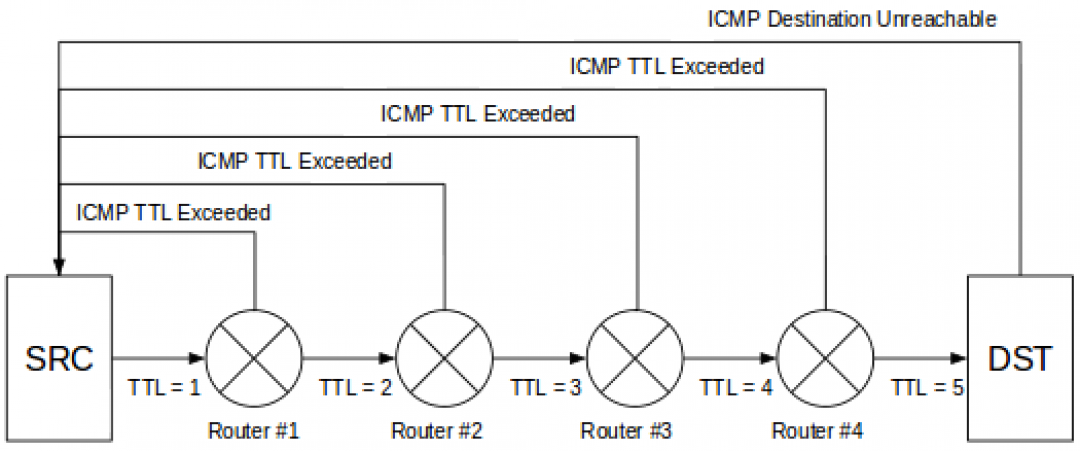
\includegraphics{traceroute-diagram.png}
    \caption{Diagram of how traceroutes work}
    \label{fig:traceroute_diagram}
\end{figure}

The mechanics of a traceroute program are then a simple procedure. With $i=1$ to start, an \icmp-based traceroute program follows the below:

\begin{enumerate}
    \item Send an \icmp ping with \TTL$=i$ to the destination server.
    \item If an \icmp \ttl-expired packet is received, mark the sender as hop $i$ along the route. If a timeout is reached, skip.
    \item If an \icmp ping response is received (i.e. the destination was reached), mark the destination server as the $i$-th hop and note the time it took to receive the packet.
    \item Increment $i$ by one and repeat from step 1.
\end{enumerate}

This process produces a list of servers along the route and their associated \rtts. A sample output from the aptly-named \texttt{traceroute} utility\footnote{\texttt{traceroute} and its variations can be found on virtually every system made in recent memory. Linux distributions and Windows machines ship with command-line tools \texttt{traceroute} and \texttt{tracert} respectively, while MacOS has its own dedicated GUI application as a system tool.} is shown in \cref{fig:sample_traceroute}. The \texttt{* * *} instances on lines 2 and 10 indicate that no response was received from these hops, so \texttt{traceroute} proceeded without them.

\begin{code}
\centering
\begin{minipage}{0.33\textwidth}
    \begin{minted}{text}
 1  192.168.1.1  16.529 ms
 2  * * *
 3  96.34.83.9  26.158 ms
 4  96.34.84.212  30.452 ms
 5  96.34.2.142  31.084 ms
 6  96.34.0.51  31.012 ms
 7  96.34.0.137  27.184 ms
 8  96.34.3.89  23.049 ms
 9  96.34.148.35  28.703 ms
10  * * *
11  108.170.246.33  26.405 ms
12  108.170.246.34  24.091 ms
13  172.217.164.142 24.720 ms
    \end{minted}
\end{minipage}
    \caption{Truncated output from \texttt{traceroute google.com}}
    \label{fig:sample_traceroute}
\end{code}

    \section{Caching}\label{sec:background_caching}

RFC 7234 describes caching as the process of storing "cacheable responses in order to reduce the response time and network bandwidth consumption on future, equivalent requests" \cite{rfc7234}. Caches save frequently used resources for a given amount of time to reduce the load on upstream resources, from the origin server to internet infrastructure that provides service along the way. Several components of the internet may contain caches: the user's browser, \cdns, \dns servers, and others \cite{2019HTTPCaching}. These all work together to free up internet bandwidth and provide a smoother experience to end users.

% Browser caching
Most, if not all, web browsers implement HTTP caching, saving commonly used website resources locally \cite{Grigorik2019HTTPCaching}. For example, if users make frequent requests from amazon.com, a cache between Amazon's servers and the users may store a copy Amazon's logo as the logo does not change frequently. When amazon.com then requests the logo, the browser's cache responds with the copy, preventing the request from going all of the way to Amazon's servers. This reduces the load on the entirety of the network that would normally service the request. Of course, sometimes resources do change, so an origin server can give cacheable resources an expiration time or max-age, after which the cache should validate the freshness resource before fulfilling the request \cite{rfc7234}. 

% CDN caching - not sure if this belongs, maybe just a brief overview before the dedicated CDN section.
\todo{Sam: Expand this paragraph if necessary}
Outside of the browser, web resources are often cached by \cdns. These networks are often set up by companies that operate major websites and are intended to move the delivery of frequently accessed resources as close to end users, both in network and geographic terms.

% DNS caching
Beyond caching resources that the end user sees and interacts with, other things, like \dns results, utilize caching as well. As discussed in more detail in \autoref{sec:background_dns}, recursive \dns servers retrieve requests from other \dns servers and often cache them for responding to future requests \cite{rfc1035}. Similar to the expiration time or max-age in HTTP caching, \dns caching has a \ttl that forces the \dns resolver to request a fresh answer.
    \section{Domain Name System}\label{sec:background_dns}

\dns, a key component of internet infrastructure and connectivity, is a hierarchical system responsible for converting domain names to \ip addresses. Domain names are human-readable names used to identify servers and websites. They are easier to remember than \ip addresses, and can point to more than one address depending on geographic location or load-balancing constraints to provide higher-performance access to websites for end-users. Domain names contain one or more parts called \textit{labels}, separated by dots. The rightmost label is the \tld (e.g. \texttt{com}, \texttt{org}, \texttt{net}, etc.). The \dns hierarchy tree subdivides into "zones," with each zone containing one or more domain names and sub-domains. Databases of domain names are maintained by \dns Name Servers, which resolve domains to \ip addresses  (\cref{fig:dns_resolution}). There are two types of name servers: authoritative and recursive.

Beyond caching resources that the end user sees and interacts with, other things, like \dns results, use caching as well. As discussed in more detail in \autoref{sec:background_dns}, recursive \dns servers retrieve requests from other \dns servers and often cache them for responding to future requests \cite{rfc1035}. Similar to the expiration time  in HTTP caching, \dns caching has a \ttl that for

\begin{wrapfigure}[18]{R}{0.4\textwidth}
    \centering
    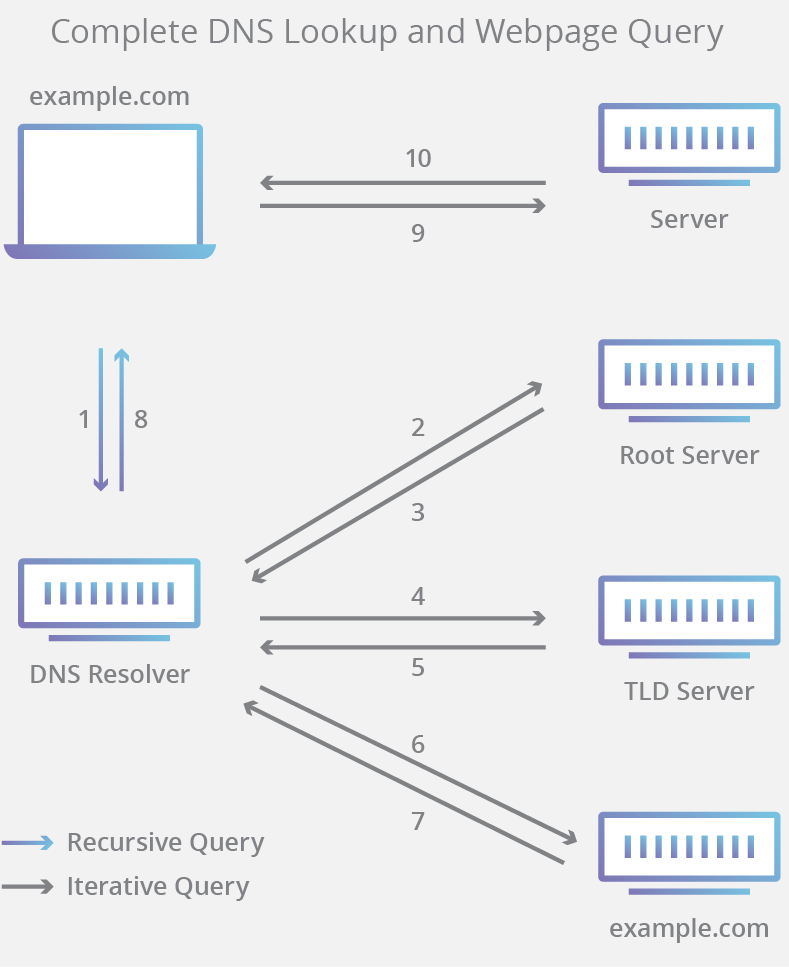
\includegraphics[width=0.4\textwidth]{images/other/dns_lookup_diagram.png}
    \caption{Diagram of DNS resolution \cite{Cloudflare2020a}}
    \label{fig:dns_resolution}
\end{wrapfigure}

\subsection{Authoritative Servers}
Authoritative servers are the primary source for the domain names within a given zone. When querying for any domain, the answer will ultimately come from the authoritative server for that domain. A \dns client can query an authoritative server directly, but it is more common that an authoritative server will be queried by a recursive server on behalf of a \dns client.

\subsection{Recursive Servers}
Recursive \dns servers work to find an \ip address for a client, so that the client does not have to do the leg work of searching through other \dns servers \cite{Cloudflarea}. \DNS resolvers use a predetermined upstream recursive \dns server, such as one provided by an \isp \cite{Oracle2010RecursiveWork}. This server then checks its cache and, if it has a valid answer, returns it. Otherwise, the server makes a series of iterative queries in order to find the requested name. 

Take for example, \texttt{www.google.com}. If the recursive server has no knowledge of any parts of the \acUrl, it will first query a pre-configured root \dns server for the authoritative server for the \texttt{.com} \tld. It will then query that server for \texttt{google.com}, then query the server provided from that request for \texttt{www.google.com} itself. At this point, the iterative component of the lookup is complete. At each stage of this process, the recursive server caches the results of its query, and assuming the \ttl has not expired, will use that cached value instead of making a fresh query. Finally, the recursive server then returns the \ip address it located, completing the recursive request from the user.

\subsection{Public Recursive \dns Servers}
An important part of this project involves public recursive \dns servers. These servers are \dns servers configured to respond to requests from anyone. Whereas most \isp servers do not advertise their \dns servers to non-customers, public servers do. Some organizations, like Google and CloudFlare, provide public \dns services because they believe doing so improves the browsing experience for end users \cite{GoogleIntroductionDNS}. These provide the public with \dns options outside of their \isp and provide this project with an important set of geographically diverse servers.

    \section{Content Delivery Networks}\label{sec:background_cdns}
\CDNs are used by many popular websites across the Internet to deliver content quickly and efficiently to their end users. \CDNs are made of data centers that are distributed across the world. These data centers are often located near large population centers or elements of the internet backbone. Some \cdns are even run by an \isp itself, primarily to help alleviate strain on their infrastructure. Content owners, such as Netflix or Reddit, pay \cdn providers to host their content on the \cdn's servers around the world to serve content more efficiently to the end users. One of the drawbacks of \cdns are that they can make it more difficult to update content stored within. As a result they are often used for static content that doesn't get updated very often, such as videos for Netflix or user content that is posted to Reddit. One example of a such a map can be seen in \cref{fig:example_cdn}.

\begin{figure}[h]
    \centering
    \missingfigure{Reddit (or other) CDN diagram}
    % \includegraphics{}
    \caption{Diagram of an example CDN}
    \label{fig:example_cdn}
\end{figure}
    \section{IP Geolocation \& Reverse Geocoding}\label{sec:background_geolocation}
Geolocation services for this project are provided by two sources: Texas A\&M University's reverse geocoding \api, and the MaxMind GeoIP2 database.

The MaxMind database is a set of binary files and an \sdk designed to estimate the location (with a \textapprox50 kilometer resolution) of an \ip address, provided by the company MaxMind. This process is referred to as \textit{\ip geolocation}. The database s imperfect\footnote{Inaccuracies are less a result of quality of data and more a result of the fact that \ip address allocation doesn't follow a meaningful geographic pattern.} but is regarded as best-in-class and is suitable for our use. Unfortunately the database is proprietary, so we have no information on how exactly MaxMind assembles and verifies it.

The Texas A\&M \api provides a reverse geocoding service that converts a set of existing coordinates into a city, state, zipcode, or other information. This is accomplished using open reference data sets (used in reverse; the normal function is to map city/state/zipcode into coordinates) and algorithms to efficiently query the database.

    \section{Prior Work}\label{sec:background_prior_work}

There have been several past attempts at evaluating \us internet connectivity, including an \mqp several years ago.

\subsection{FCC fixed broadband deployment map}
The \FCC maintains a map of broadband internet deployment across the United States \cite{FederalCommunicationsCommission}. This map is drawn at a census block level and only considers residential broadband.
 
 \subsection{Internet Connectivity MQP 2018}
In 2018, another \mqp was run at \wpi, also with the goal of mapping the internet connectivity across the United States. They used traceroutes from Worcester to top websites, and also performed \dns cache manipulation to collect their data. They had mixed success collecting data, but they were ultimately able to produce a map of all their \dns data interpolated to cover the entire \us, shown in \cref{fig:interpolated_dns_map}. They did not come to any conclusions as to the best or worst states \cite{Fakult2019}.

The core concept of \dns cache manipulation was ultimately used in our own research into evaluating and ranking internet connectivity, discussed in \cref{sec:dns}.

\begin{figure}[h]
    \centering
    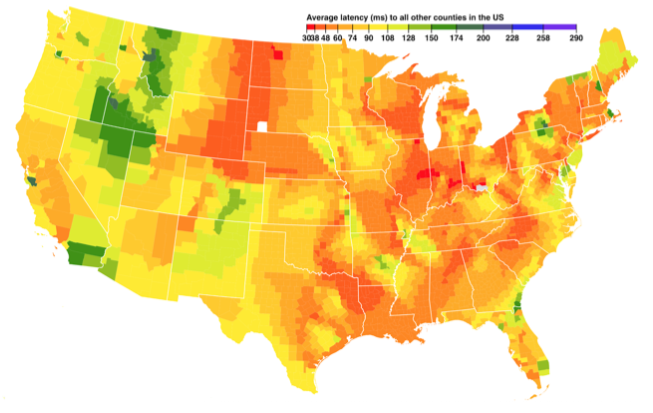
\includegraphics[width=\textwidth]{dns/prior_mqp/dns-map.png}
    \caption{Interpolated DNS map}
    \label{fig:interpolated_dns_map}
\end{figure}
 
\subsection{Physical Mapping of the Internets Fiber Backbone in the United States}
In 2015 researchers at the University of Wisconsin (Madison) set out to map the locations of the fiber backbone within the \us.  Their goal was to understand how the physical locations of the fiber backbone had been influenced by previous infrastructure such as railroads and the highway network. They found strong correlation between the location of fiber lines and the locations of major roads built in the mid 20th century. This result is significant for internet connectivity because it further highlights that cities that were well connected physically during the industrial revolution continue to be the best connected.
 
    
    \newpage
    \chapter{Design}\label{sec:design}
    Internet access is an increasingly important part of the American economy and everyday life. Functions as simple as applying for a job, keeping in touch with friends, or continuing self-education all require internet connectivity. Major technology firms are often in the public spotlight, and common internet services can be found everywhere in public, ranging from music and video streaming, to online e-book stores, to digital storefronts. For a more quantitative evaluation, in 2018 an industry group comprised of major technology firms estimated that the "internet sector" of the economy alone represented \$2.1 trillion a year, or about 10\% of the \us economy \cite{Shepardson2019InternetGroup}.

Unfortunately not all parts of the \us are as well connected as others, even by measures from simple personal anecdotes. For instance, it is  quite possible to find a town in rural Indiana where the best connection isn't good enough to stream a movie, while driving just 45 minutes east will yield a connection an order of magnitude better. Subjective measures and tales like this are common everywhere across the \us, but there is little scientifically-rigorous or complete data available. For instance, the \fcc has a map of estimated broadband deployment \cite{FederalCommunicationsCommission}, but simple broadband deployment isn't necessarily a good measure of how well connected people in those areas actually are.

To address these problems, we set out to gather and analyze as much data as we could on how well connected Americans are to the internet, using various means and measures. Our hypothesis is simple: although there may be some regional variations or "spottiness," there is a relationship between your location in the \us and what sort of internet service you can expect. We hypothesized that areas near each other are likely to have similar connectivity to one another, and that these similarities will form large scale trends that should be visible on a map, both visible and interpretable by non-technical readers.

The end goal of our project was to find if such relationships exist, and if so, to conduct analyses on the data to make the differences between areas of the \us clear. An important quality of our work is that it should be scientifically rigorous and statistically valid -- that is, we should avoid systemic error and account for random error in our calculations -- so a great deal of effort was expended on ensuring the validity of our results.

The reminder of the report is organized into chapters as follows:

In \cref{sec:background} we present background information on the fundamentals of the internet, information relevant to our methods, and research conducted on prior works and attempts at measuring connectivity.

In \cref{sec:connectivity_defs} we rely upon collected background research to define some metrics for internet connectivity. These are not limited to traditional metrics used by consumers (such as speed), instead taking a more expansive approach.

\Cref{sec:methods} describes a brief overview of our three main methods for collecting \& analyzing data on internet connectivity. We also present a brief overview of some of the statistical methods used, and an explanation of some methods that were considered but ultimately rejected.

\Crefrange{sec:caida}{sec:dns} present detailed methods of the design, implementation, and analysis for each of our three methods for collecting data. Their analyses differ since each dataset is somewhat different, but the fundamentals (e.g. definitions of connectivity) remain largely the same.

\Cref{sec:comparative_analyses} contains our comparative analysis of the results of the three data analyses. We present overall conclusions drawn from the data, in both things we assert we are confident of and things we assert we are uncertain of.

Finally, in \cref{sec:future_work} we suggest ideas for future projects to follow up on, drawing from shortcomings noted in our methods and the unpursued methods explained in \cref{sec:methods}.

\todo{Should we include the conclusion in the roadmap?}

    \section{Web Ping}\label{sec:design_web_ping}
\textit{Assigned to: Evan}

% General overview / introduction

% Operating principles
    % Loading small resources
    % Back-to-back calls to investigate TCP keep alive
    % Geolocation
        % Primary: IP geolocation
        % Secondary: User provided via browser
    % Determining connection type
    
% Distribution and collection
    
% Data
    % Type
    % How is it useful? To who?
    
    \section{DNS Cache Manipulation}\label{sec:design_dns}

\subsection{Approach overview}
\dns cache manipulation makes use of two sets of geographically diverse \dns servers: one list each of recursive and authoritative servers. The basic principle rests on the concept of making requests directly to each of the recursive servers that \textit{must} make their way to the authoritative ones and deducing the time between the two. As \dns includes no mechanism for reporting the time taken between two servers, \dns cache manipulation must rely on the \rtt from when the local request is dispatched to when an answer is received.

\subsection{Collection Stages}\label{sec:dns_design_collection_stages}

\subsubsection{Confirmation of Server Status and Type} 
Prior to running any tests, two lists of candidate recursive and authoritative servers are fed into tools that confirm their status as usable servers. For recursive servers, this process confirms that they are indeed public recursive servers. For authoritative candidates, it verifies that the server provides an answer for the domain it is expected to.

\subsubsection{Testing Reliability}
\todo{A diagram or two would definitely help. Also CoV def.}
Before actually using any of the servers for testing, we tested their reliability -- i.e. how consistent their response times were under constant parameters. After making repeated requests to each server, that in theory should have similar response times, we filter servers based on the Coefficient of Variation for the measured response times. This eliminated any servers with high variation from the testing. For recursive servers, priming the cache (see below) and then making repeated requests for the primed value served as the repeated requests. For authoritative servers, this was accomplished by making repeated requests for a random subdomain that the servers are authorities for through the WPI recursive \dns server. This server is close enough to the machine we ran the tests on that the lag was minimal. The justification for running the filtering prior to testing is that each server included in the test increased the time required to run the entire test suite exponentially, as each recursive server was paired with each authoritative server.

\subsubsection{Priming the DNS Cache} 
The first step of the actual testing involves priming the target recursive server's cache. Say the target recursive server's \ip address is \texttt{1.2.3.4} and the target authoritative server provides answers for \texttt{example.com}. By making a \dns query to \texttt{1.2.3.4} for \texttt{example.com}, we get the target \dns server to cache the answer to the query.

\subsubsection{Measuring Latency} 
After the target recursive server has cached the answer for the query for \texttt{example.com}, it will use that cached answer to respond to subsequent requests without making any iterative requests. We can then make another request, identical to the one in the priming stage, and time it. To get a latency measurement, we do this several times back to back and take the lowest value, which indicates the best possible latency between the machine the measurements are being taken on and the recursive server.

\subsubsection{Measuring the Total RTT} 
The final step in the process is to measure the \rtt between the local machine and the target authoritative server and subtract the latency to get the final result. To do this, we make a query to the recursive server for \texttt{random.example.com}, where \texttt{random} is a randomly generated sub-domain that is unlikely to actually exist on the targeted domain. This random sub-domain forces the recursive server to get an answer. Because it already knows the authoritative server for \texttt{example.com}, it can skip the process of querying the root and \texttt{.com} servers and make an immediate query to the server for \texttt{example.com}. We measure the time for this entire process and then subtract the previously measured latency, leaving only the time between the target recursive server and the target authoritative server, which is recorded.
    
\textcolor{red}{Probably put a diagram (like the one from the poster) here.}

\subsection{DNS Server Lists}

Initial lists of both types of \dns servers were provided to us by our advisor, Professor Craig Wills. After verifying the status of these servers, we augmented the list by searching through a list of `.gov` domains filtered by the states we needed to fill in gaps for. In total, this lists included 535 authoritative servers and 1225 recursive servers.

Of note, the final list of recursive servers did not include any servers located in the state of Rhode Island despite a rather extensive search for such a server.
    \section{CAIDA \& Atlas Measurements}\label{sec:design_caida}\todo{Proofread and trim down phrasing}

As discussed in \autoref{sec:background_connectivity}, one way to measure internet connectivity is by an everything-to-everything approach where the \rtt between as many devices in a region as possible is measured. Collection of such data requires either moving one device to many places or having an enormous network of devices distributed across the globe; in either case the device(s) would ping as many different devices as they can find.

Fortunately such projects exist --- two organizations, \caida and \ripe maintain projects that do almost exactly that. \caida and \ripe (the latter through its Atlas project) have networks of thousands of small network-connected devices, typically Raspberry Pis or similar, that scan vast swathes of the internet, constantly running \gls{traceroute}s (see \autoref{sec:background_traceroutes}). For example, \caida's project involves a technique they call "prefix probing" whereby the \caida data collection network tries to run a \gls{traceroute} to at least one device in every /24 prefix. Together these networks have generated terabytes of data over many years, all of which is publicly available.\footnote{\CAIDA's prefix probing data can be found at \url{https://www.caida.org/data/active/ipv4_prefix_probing_dataset.xml}. The \ripe Atlas dataset may be found at \url{https://data-store.ripe.net/datasets/atlas-daily-dumps}}

\subsection{Direct Ping Calculation}

Since a \gls{traceroute} is really just a series of pings, and traceroute output reports the \rtts for all of them, \caida and \ripe Atlas traceroute data can be used for the everything-to-everything \rtt approach. The methodology is simple: for every hop in each traceroute, record the source, the destination, and the \rtt. IP geolocation can be used to determine source and destination coordinates, and the Haversine formula can be used to find a distance between them (formula \ref{form:haversine_distance}). This technique is referred to as \textit{direct ping calculation}.

\begin{formula}
    \begin{equation}
        d = 2r\arcsin{\sqrt{\sin^2{\left(\frac{\rho_2-\rho_1}{2}\right)} + \cos{\rho_1}\cos{\rho_2}\sin^2{\left(\frac{\lambda_2-\lambda_1}{2}\right)}}}
    \end{equation}
    \caption{Haversine formula for distance; $\rho_1,\rho_2$ and $\lambda_1,\lambda_2$ are latitude/longitude respectively for the two points in radians, and $r$ is the radius of the Earth at 6,371 km.}
    \label{form:haversine_distance}
\end{formula}

\subsection{Indirect Ping Calculation}

Of note is that a crude calculation of the \rtt between each individual server can also be performed without directly sending pings out from it. By taking one server's \rtt and subtracting the \rtt from the server one hop behind it, we can loosely estimate how long it takes the two to communicate. For example, hop 4 in figure \ref{fig:sample_traceroute} has an \rtt of 30.452 ms while hop 3 has an \rtt of 26.158 ms. We can then estimate an \rtt of 8.588 ms between hops 3 and 4.\footnote{This is equal to \textit{twice} the value of the difference, since a simple subtraction would yield one-way communication, whereas we want \rtts.} The same technique applies to any two arbitrary pairs of hops in the traceroute log, although a sanity check to guard against negative \rtts (likely due to jitter along the connection) is needed.

This technique results in roughly double the amount of data per traceroute, since if you have a traceroute $A\rightarrow B\rightarrow C\rightarrow D$, you have data for not only $A\rightarrow B, A\rightarrow C,$ and $A\rightarrow D$, you can calculate $B\rightarrow C, B\rightarrow D$, and $C\rightarrow D$. For a traceroute of $n$ hops, you can extract $2n-2$ \rtts. This technique is referred to as \textit{indirect ping calculation}.
    \section{Methods not Pursued}\label{sec:design_unused_methods}% TODO: Better name?

\subsection{Road trip}

Before the \caida and \ripe Atlas data was uncovered, an idea for gathering everywhere-to-everywhere data was conceived and seriously considered: take an enormous road trip across the United States, taking measurements along the way. The idea is simple enough in theory and in practice. Just assemble a list of websites to run traceroutes to and run constant traceroutes against them on the journey, mapping them to GPS coordinates along the way.

By the end of the trip there would be traceroutes from every point along the route to all the different sites in the list, many times over. This, it was hoped, would yield a significant amount of quality data. With two people in one car taking shifts in driving (or alternately, staying in hotels for 7-8 hours at a time), it was estimated that the entire US could be roughly circumnavigated in about 7 days.

Fortunately the \caida and \ripe Atlas data sets were discovered well before any serious planning was underway. The idea was almost immediately nixed, since it turns out that nobody actually wants to spend a week in a car.

\subsection{Network Time Protocol}

\ntp is a protocol designed to keep computer clocks around the world in sync with each other. Per the specification for the third version, \ntp is designed to "maintain accuracy and robustness" despite being implemented on "unreliable" networks with "dispersive delays" \cite{rfc1305}. As part of this protocol, the delay, or delta, between the client and server is calculated \cite{rfc5905}. Given the precise nature of this protocol, it would be ideal for this project, which is focused on measuring the network time between geographic locations. The only requirements would be a geographically diverse set of \ntp servers willing to provide the calculated delay values to their peers. Luckily, both parts of this requirement are met -- sort of.

The \ntp specification details a server mode, mode 6, that allows for "remote control queries" which provide a way for remote management of certain aspects of the server \cite{Haberman2019Control4}. One of the these queries, the \texttt{peers} command, prompts the server to return a list of its peers, along with calculated statistics for these peers -- including the delay. \autoref{fig:sample_ntpq} is an example of such a command using the \texttt{ntpq} tool (with some returned fields removed for formatting).

\begin{figure}[h]
    \centering
    \begin{minted}{bash}
    >ntpq -c peers 127.0.0.1
         remote           refid      delay   offset  jitter
    =======================================================
    *ntp1.wpi.edu    130.215.32.36   0.851   -0.076   0.134
    +ntp2.wpi.edu    130.215.32.36   0.646   -0.366   0.182
    +ntp3.wpi.edu    130.215.144.33  1.376    0.711   0.261
    \end{minted}
    \caption{Sample NTP Mode 6 \texttt{peers} command output}
    \label{fig:sample_ntpq}
\end{figure}

As the example shows, the \texttt{peers} command response includes both the delay and the jitter calculations for each peer. Coupled with \ip geolocation, requesting the peers from a list of mode 6 \ntp servers would be a straightforward way of getting point to point measurements. And there is no shortage of \ntp servers with mode 6 enabled in the United States: according to the ShadowServer Foundation, which conducts period scans for such servers, as of January 22nd, 2020, there are 522,415 such servers in the country \cite{TheShadowserverFoundationNTPProject}. Additionally, as \autoref{fig:ntp_mode_6_us_map} shows, they are distributed across most of the country.

\begin{figure}[H]
    \centering
    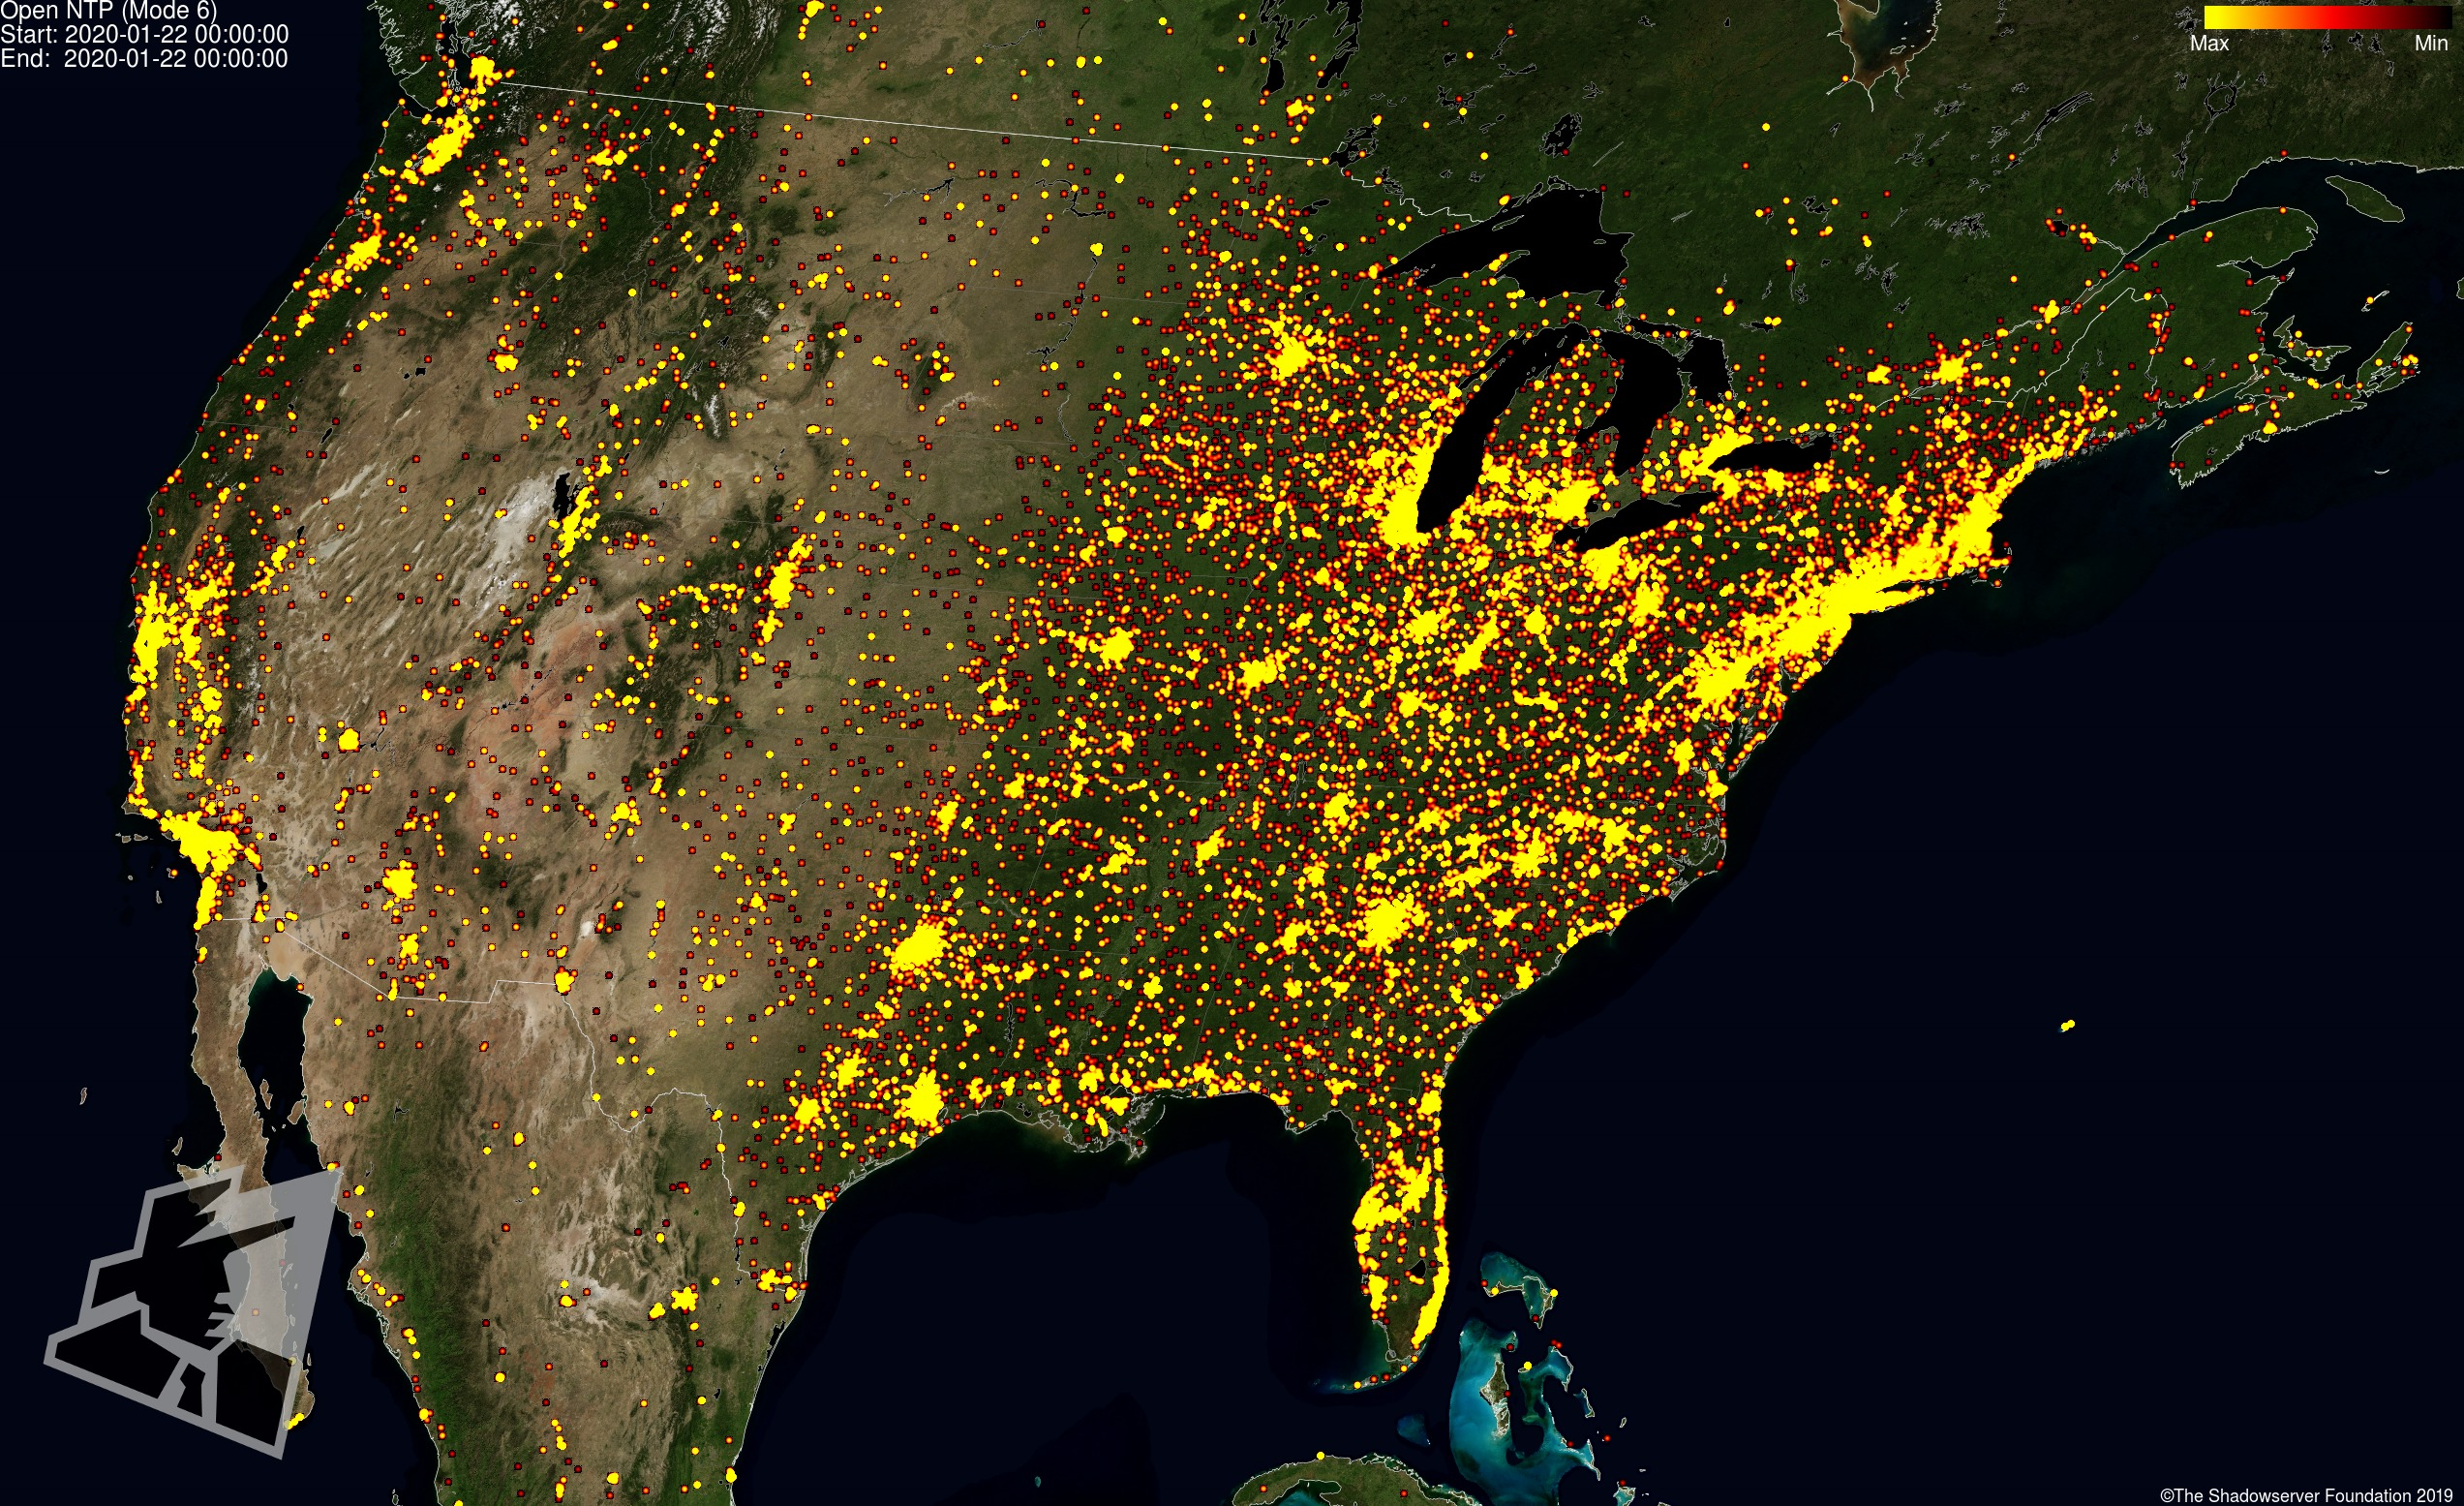
\includegraphics[width=\textwidth]{images/ntpversion_united_states_current.jpg}
    \caption{Distribution of \ntp Mode 6 Servers in the US}
    \label{fig:ntp_mode_6_us_map}
\end{figure}

In theory, using these servers and conducting a simple survey of the delay times to each of their peers would be an ideal method for this project. Unfortunately, one of the commands included in mode 6 makes the servers vulnerable to being exploited for use in amplified \ddos attacks \cite{USDepartmentofHomelandSecurity2014NTPCVE-2013-5211}. Thus, despite performing frequent scans for mode 6 servers, the ShadowServer Foundation does not publish a list of such servers, since doing so would be a security risk. We found no other source of potential servers and proceed to attempt our own scan of potential \ip ranges. While we found some potential servers, many lacked any peers and the search was time intensive. Future work may include this method, as it is promising, provided a list of potential servers is available, or more time can be dedicated to scanning for them.

\subsection{ISP Mapping}
FCC fixed broadband deployment map
 The \FCC maintains a map of broadband internet deployment across the United States \cite{FederalCommunicationsCommission}. This map is drawn at a census block level and only considers residential broadband.

    \section{Putting it all Together}\label{sec:design_cumulative} % TODO: Better section name?

    
    \newpage
    \chapter{Implementation}\label{sec:implementation}
    \section{Web Ping}\label{sec:web_ping_impl}
\subsection{Website}
\subsection{Distribution}
    \section{DNS}\label{sec:dns_impl} % TODO: More descriptive name?
    \section{CAIDA \& Atlas Processing}\label{sec:caida_impl}\todo{Proofread and trim down phrasing}

A website scrape of as much \caida and \ripe Atlas data as a teammembers' hard drives could handle was taken using the common tool \texttt{wget} (and later an http-accelerator program \texttt{axel}). \ripe Atlas data is stored in \json format while \caida developed its own binary format "WARTS" for more efficiently storing data. While the code for reading it is open source, a toolkit including a warts-to-\json converter is available for download\footnote{\url{http://www.caida.org/tools/measurement/scamper}} and once converted the resulting \json file is similar to the \ripe Atlas format. This enabled development of an all-in-one \etl program to process both file formats and combine their data into one large database. The total volume of data processed is estimated at 5-10 terabytes.

\subsection{Data ETL Pipeline}

The pipeline was implemented as a bash script that operated in three stages. This process was designed to be highly parallelizable and so the aptly-named \texttt{parallel} tool \cite{Tange2011} was used to process 8-16 files at a time.

\paragraph{Extraction} \ripe Atlas distributes data in compressed (gzip) format, each of which contains a single 10 GB \json file. \caida distributes files in compressed WARTS format, which expands to 3 GB \json files when unloaded and converted. These files were extracted and converted as necessary on a ramdisk to speed up processing. Since 10 GB files are unwieldy and the file format permitted it, \ripe Atlas files were split into chunks of 100,000 traceroutes each -- about 3,000 files total.

\paragraph{Transformation} A program (dubbed the "traceroute hopper" program while in development) was developed in C++ to parse the \json files and perform direct+indirect ping calculations for each traceroute (see \autoref{sec:design_caida}). C++ was chosen for its performance\footnote{Python was originally used but suspected to be slow; switching to C++ yielded a 100\% performance boost, saving several days of processing time.} and availability of \json parsing libraries. Internally the program scans line by line through traceroute files, performs necessary calculations to determine \rtts (and in the case of \caida data, occasional \dns resolution), and stores the results in a configurable internal buffer.\todo{Add a reference to the appendix so the code for the traceroute hopper can be found}

\paragraph{Load} Once the traceroute hopper reaches its buffer's capacity it dumps the contents out to a PostgreSQL database. PostgreSQL was chosen for its performance, advanced features, and in particular its ability to generate spatial indexes, valuable to the \gis oriented work this project involved. Performing basic statistical analyses and joins was also a sought-after feature.

\bigskip

Once all data was collected in the database it was possible to sort out unique \ips, each of which was fed into a geolocation library (see \autoref{sec:background_geolocation}) provided by MaxMind to estimate the location of the machine the \ip address belonged to. This step was delayed until after the main \etl process for performance reasons. After processing was completed, the database contained \textapprox71,000,000,000 individual \rtt measurements.

\subsection{Data Cleaning \& Initial Processing}

The data required some cleaning before it could be considered viable for serious analysis. For unknown reasons, some collected \rtts were \textit{extremely} large, on the order of hundreds of thousands of milliseconds, so some filtering was needed on individual measurements. Some servers also showed a consistent tendency towards exceptionally high \rtts (several thousand milliseconds) in a manner that was inconsistent with others, so these too were filtered out (potentially discarding dozens of measurements at a time). Since threshold filters (ex. removal of all points above $x$ ms) risk biasing data, simple Z-score filtering was selected -- values with an absolute Z-score above 2.0 were discarded.

After cleaning the data was grouped together by source-destination \ip pair. Many pairs had multiple measurements each, so for each the range, the average, standard deviation, measurement count, and range were calculated. This grouping processed also assigned coordinate pairs to each IP pair, enabling geographic processing. After grouping there were \textapprox230,000,000 data points.

    
    \newpage
    \chapter{Results}\label{sec:results}
    \section{Web Ping}\label{sec:results_web_ping} % TODO Better section name?
    \section{DNS}\label{sec:dns_results} % TODO Better section name?
    \section{CAIDA \& Atlas Analyses}\label{sec:caida_results}\todo{Proofread and trim down phrasing}

Once data \etl was complete, analysis in earnest was possible. The following sections describe analysis of the \caida and \ripe Atlas data in a natural progression from analysis of data quality, to basic connectivity analysis, and finally to geographic plotting and \gis tooling.

\subsection{Data Quality}

To gain a better understanding of the quality of the data, a series of charts were made using kernel density estimation with a Gaussian kernel. These charts should be read in a similar fashion to probability distribution functions.

\begin{figure}[H]
    \centering
    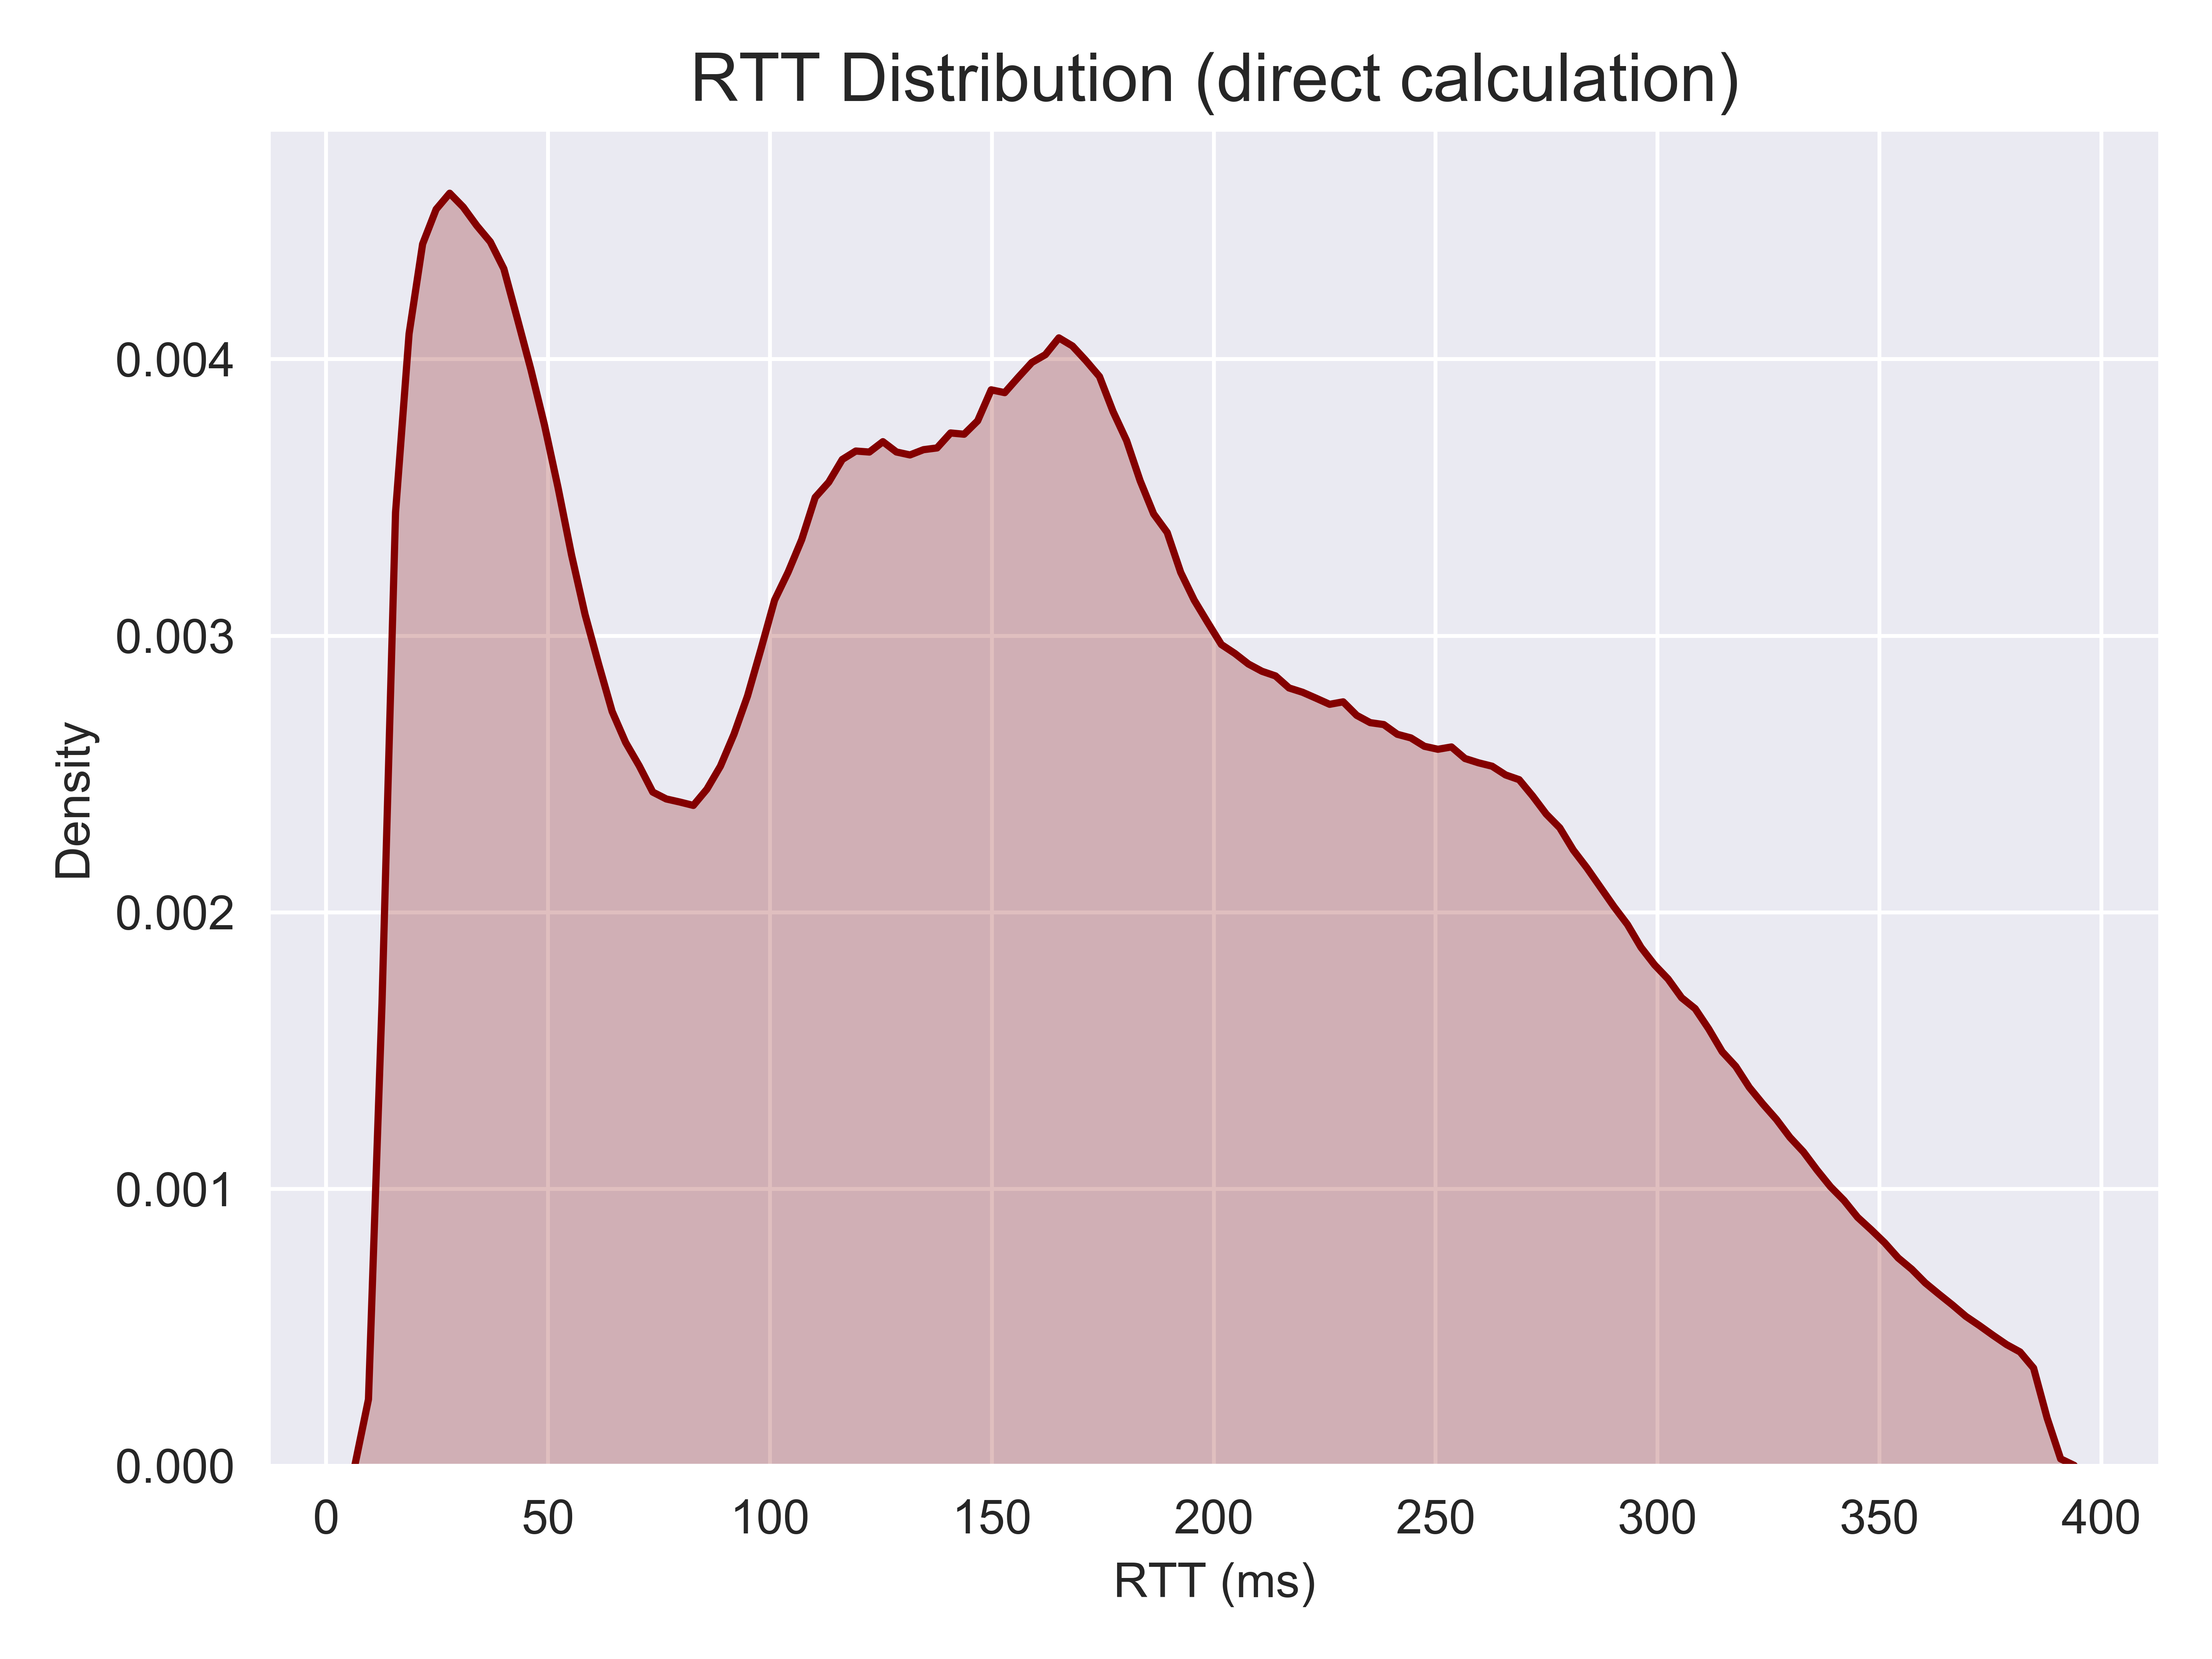
\includegraphics[width=0.75\textwidth]{caida/rtt_distribution.png}
    \caption{Distribution of RTT between IP pairs, direct ping calculation}
    \label{fig:caida_rtt_distribution}
\end{figure}\todo{Fix chart placement}

The most immediately useful distribution is that of the \rtt between \ip pairs, shown for direct-calculated \rtts in \autoref{fig:caida_rtt_distribution}. The distribution appears weakly bimodal, which we hypothesize is due to the global nature of \ripe Atlas and \caida's individual measurement networks. The leftmost peak would correspond to measurements to a device that shares a land mass with the device performing the \gls{traceroute}, while the right peak would correspond to a combination of devices on a different land mass and devices with lower-performing connections. \autoref{fig:caida_distance_distribution} appears to confirm this hypothesis, since it too is similarly bimodal.

\begin{figure}[H]
    \centering
    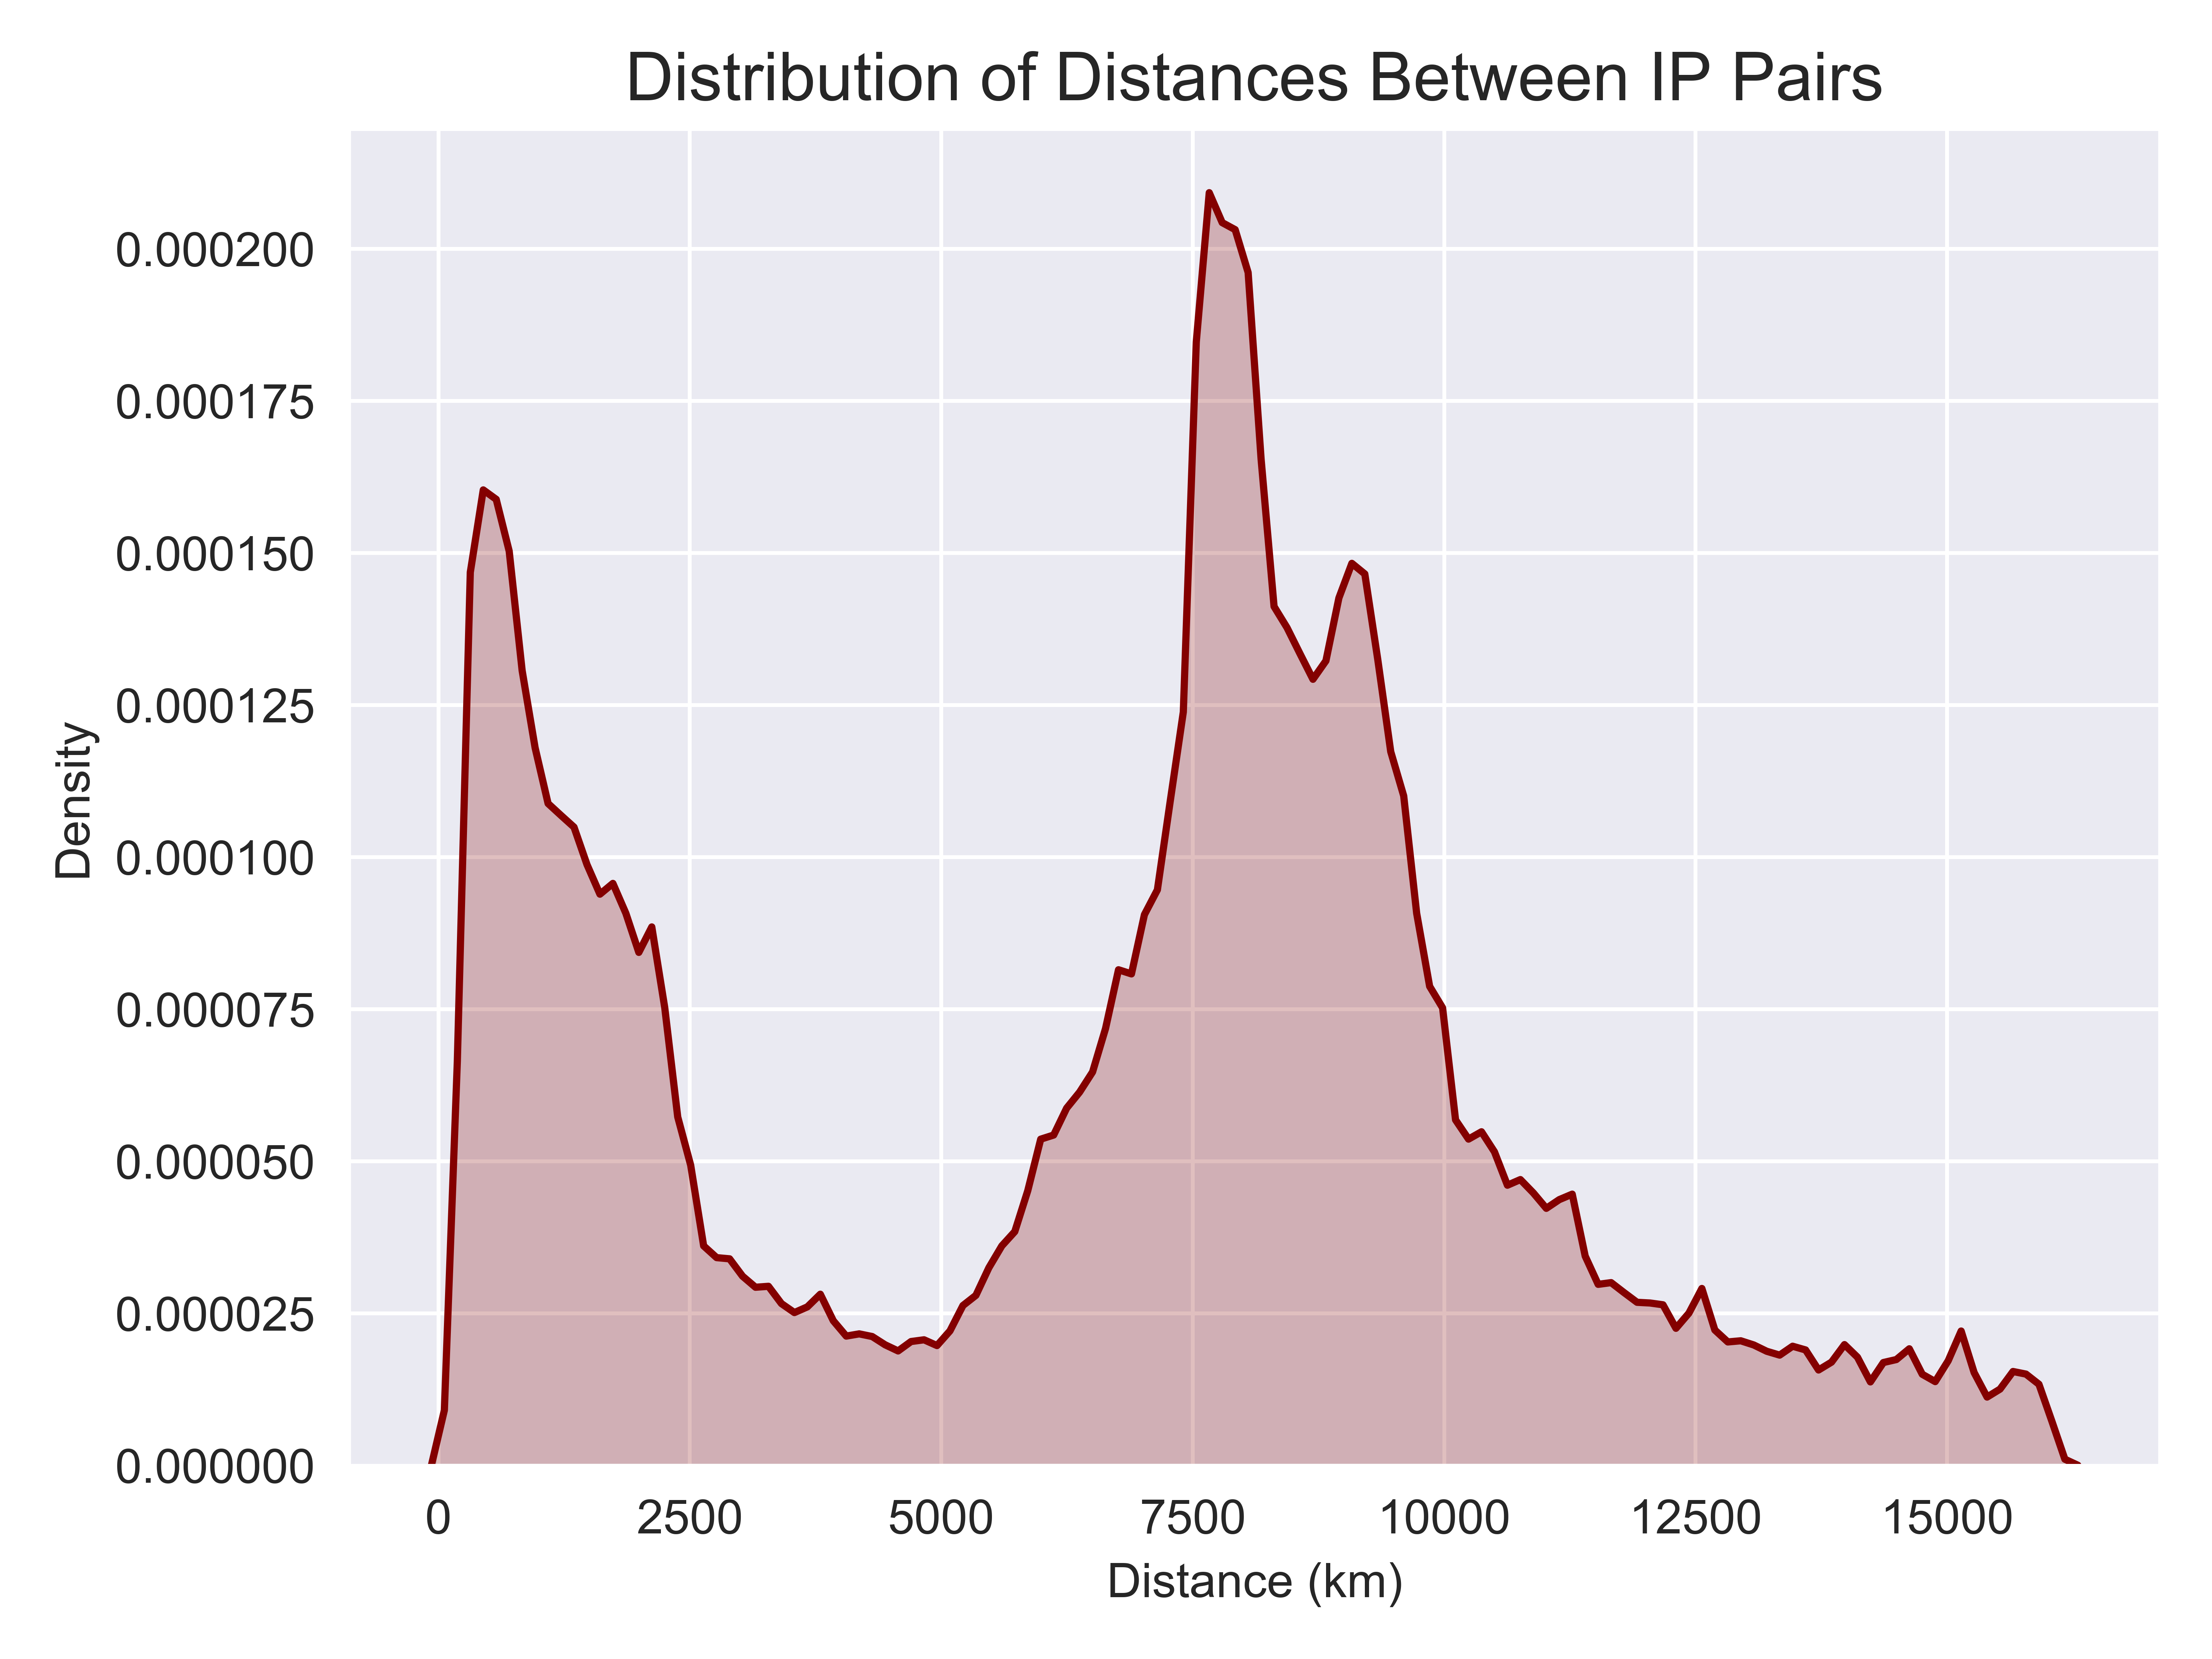
\includegraphics[width=0.75\textwidth]{caida/distance_distribution.png}
    \caption{Distribution of distance between IP pairs}
    \label{fig:caida_distance_distribution}
\end{figure}

Unfortunately the data from indirect ping calculation (see \autoref{sec:design_caida}) had to be discarded as they were deemed too unreliable. \autoref{fig:caida_rtt_distribution_indirect} shows the distribution of \rtts calculated using the indirect ping calculation method, of which a calculated \textapprox29\% are below zero. Since a significant fraction of the data points are completely impossible it was decided that this data was too reliable for further analysis. The remainder of the data analyses in this section are based on the direct ping calculation method only.

\begin{figure}[H]
    \centering
    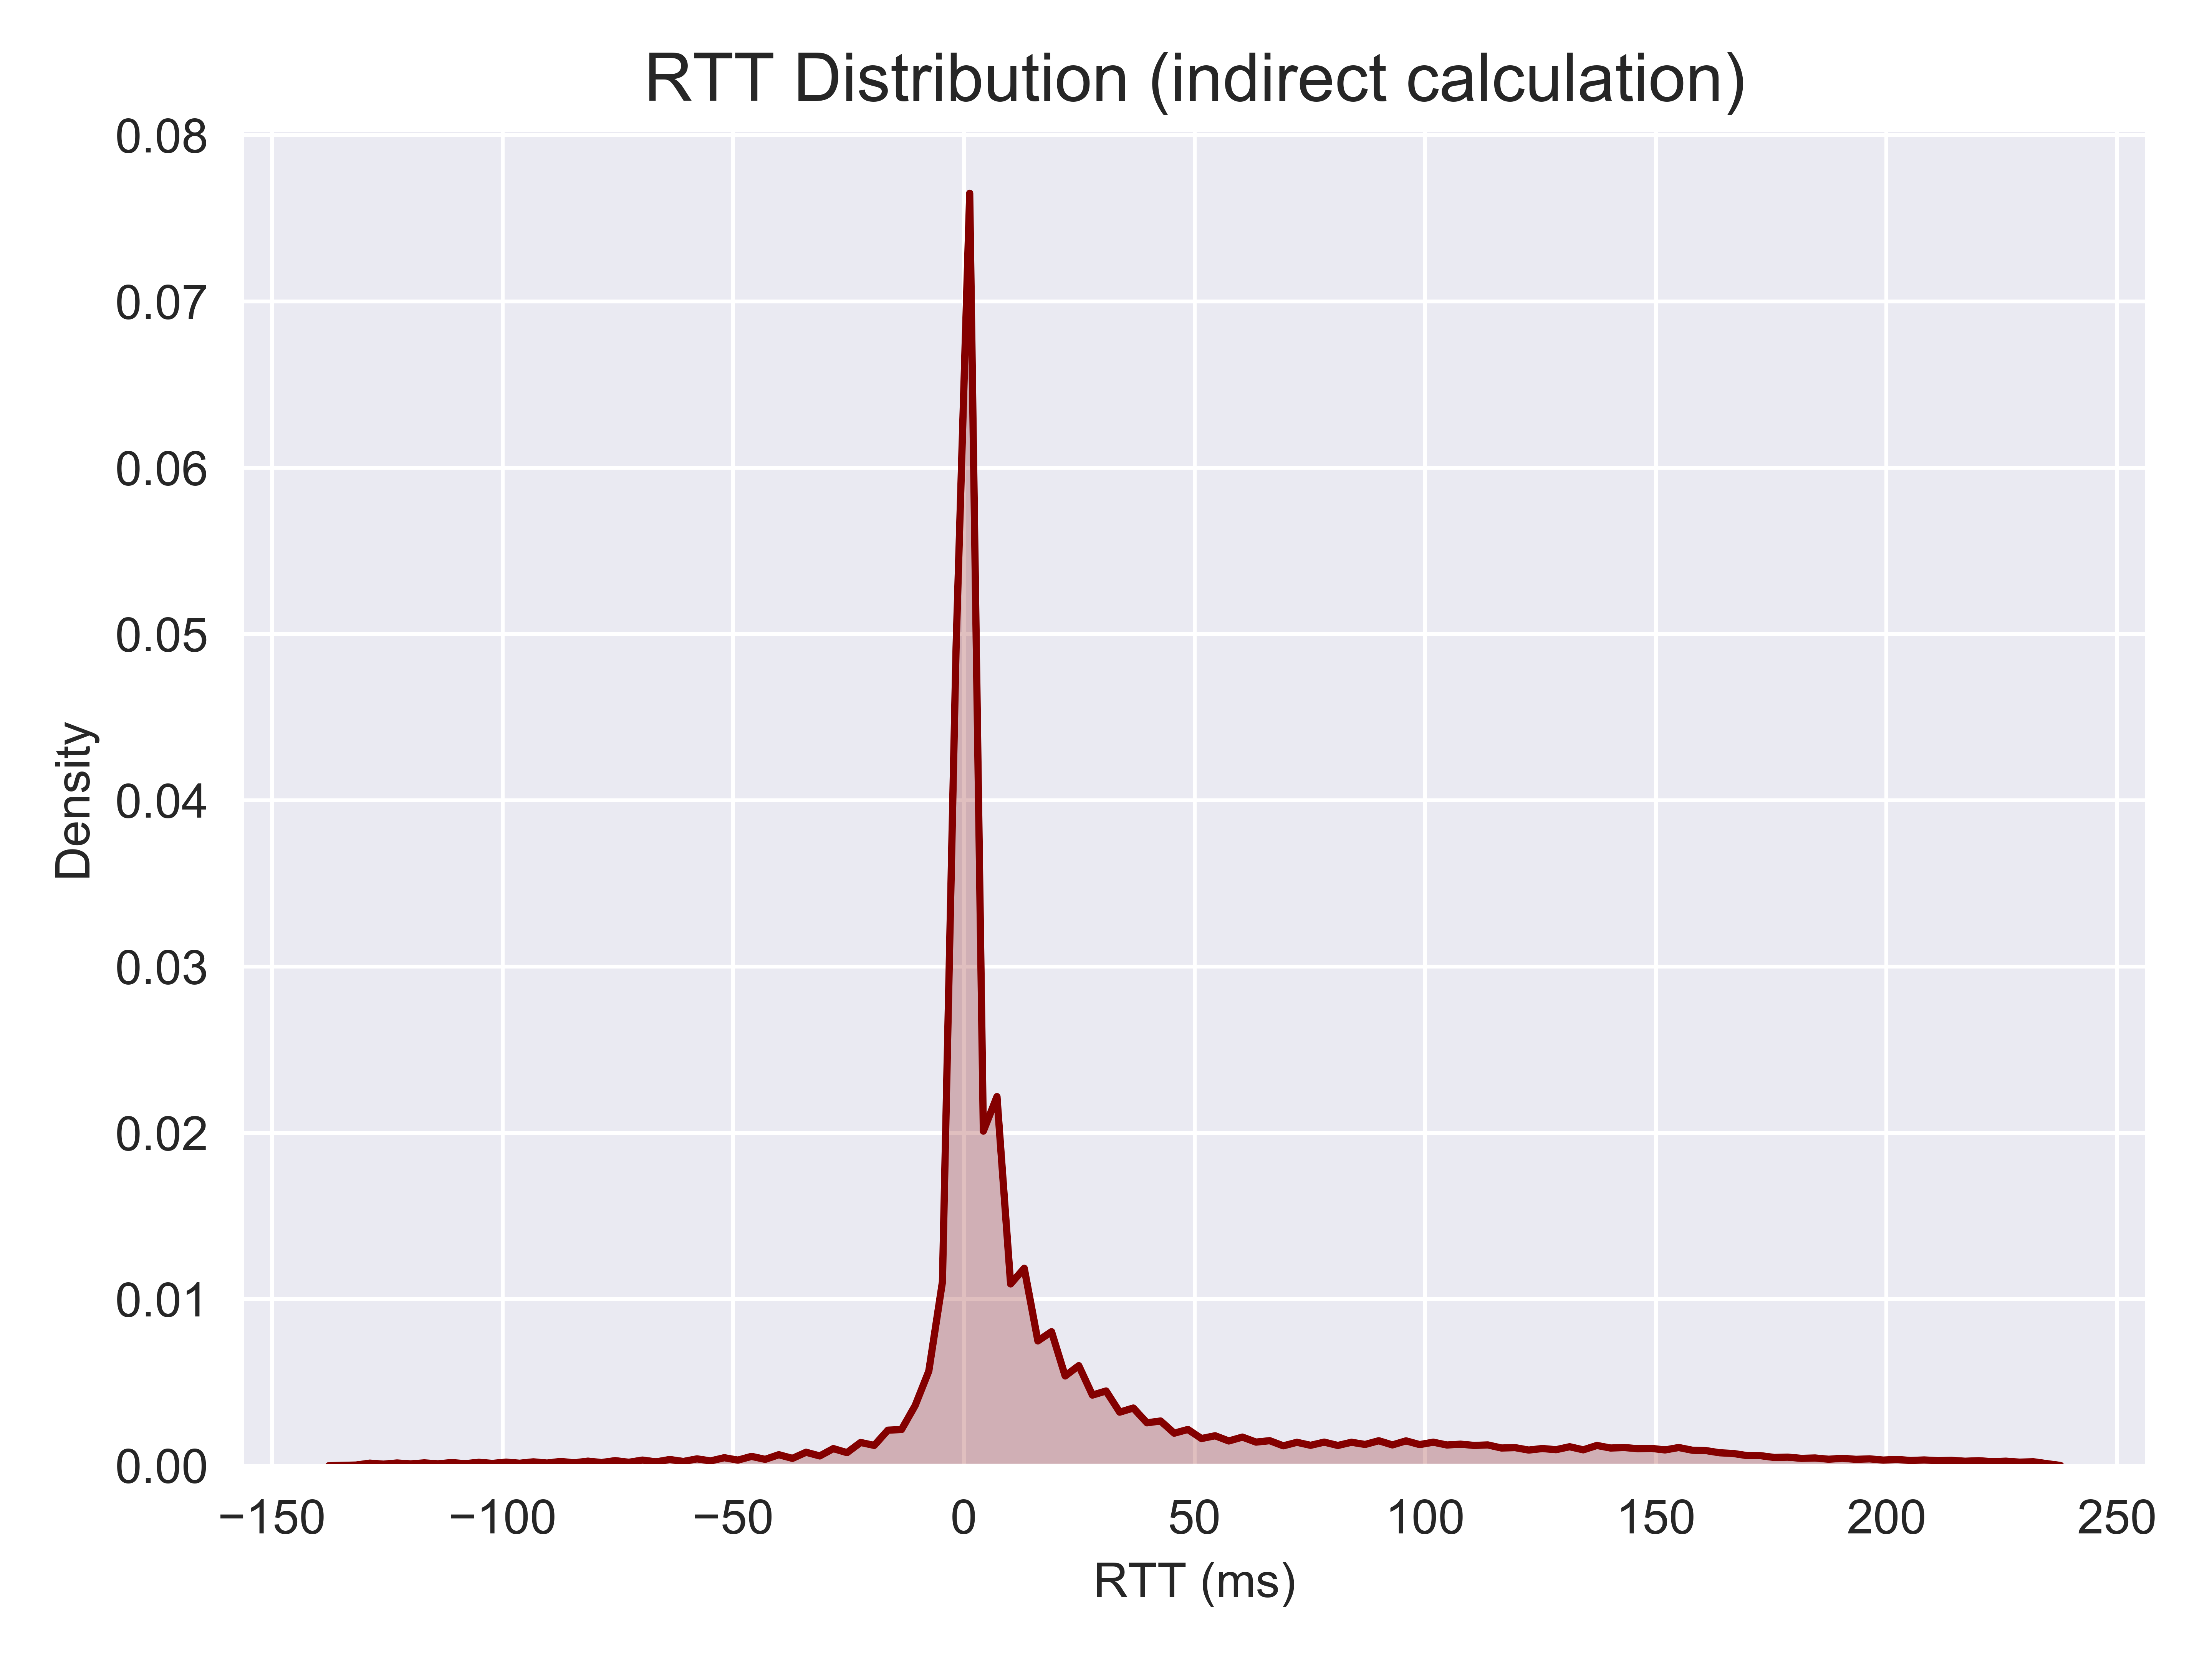
\includegraphics[width=0.75\textwidth]{caida/rtt_distribution_indirect.png}
    \caption{Distribution of RTT between IP pairs, indirect ping calculation}
    \label{fig:caida_rtt_distribution_indirect}
\end{figure}

To further assess data quality we turned to measures of the reliability of each data point. \autoref{fig:caida_measurements_distribution} shows the distribution of measurements count between each \ip pair, showing that although most \ip pairs had on the order of 1-20 measurements, a sizeable fraction had more than that, and there were even some in the 500+ measurements range. This is hypothesized to be the result of the way \ripe Atlas and \caida nodes are networked. A node's local gateway would always show up on a \gls{traceroute} (unless configured to not respond to pings) as would common paths through a node's \isp, so these \ips are likely measured extremely frequently.

\begin{figure}[H]
    \centering
    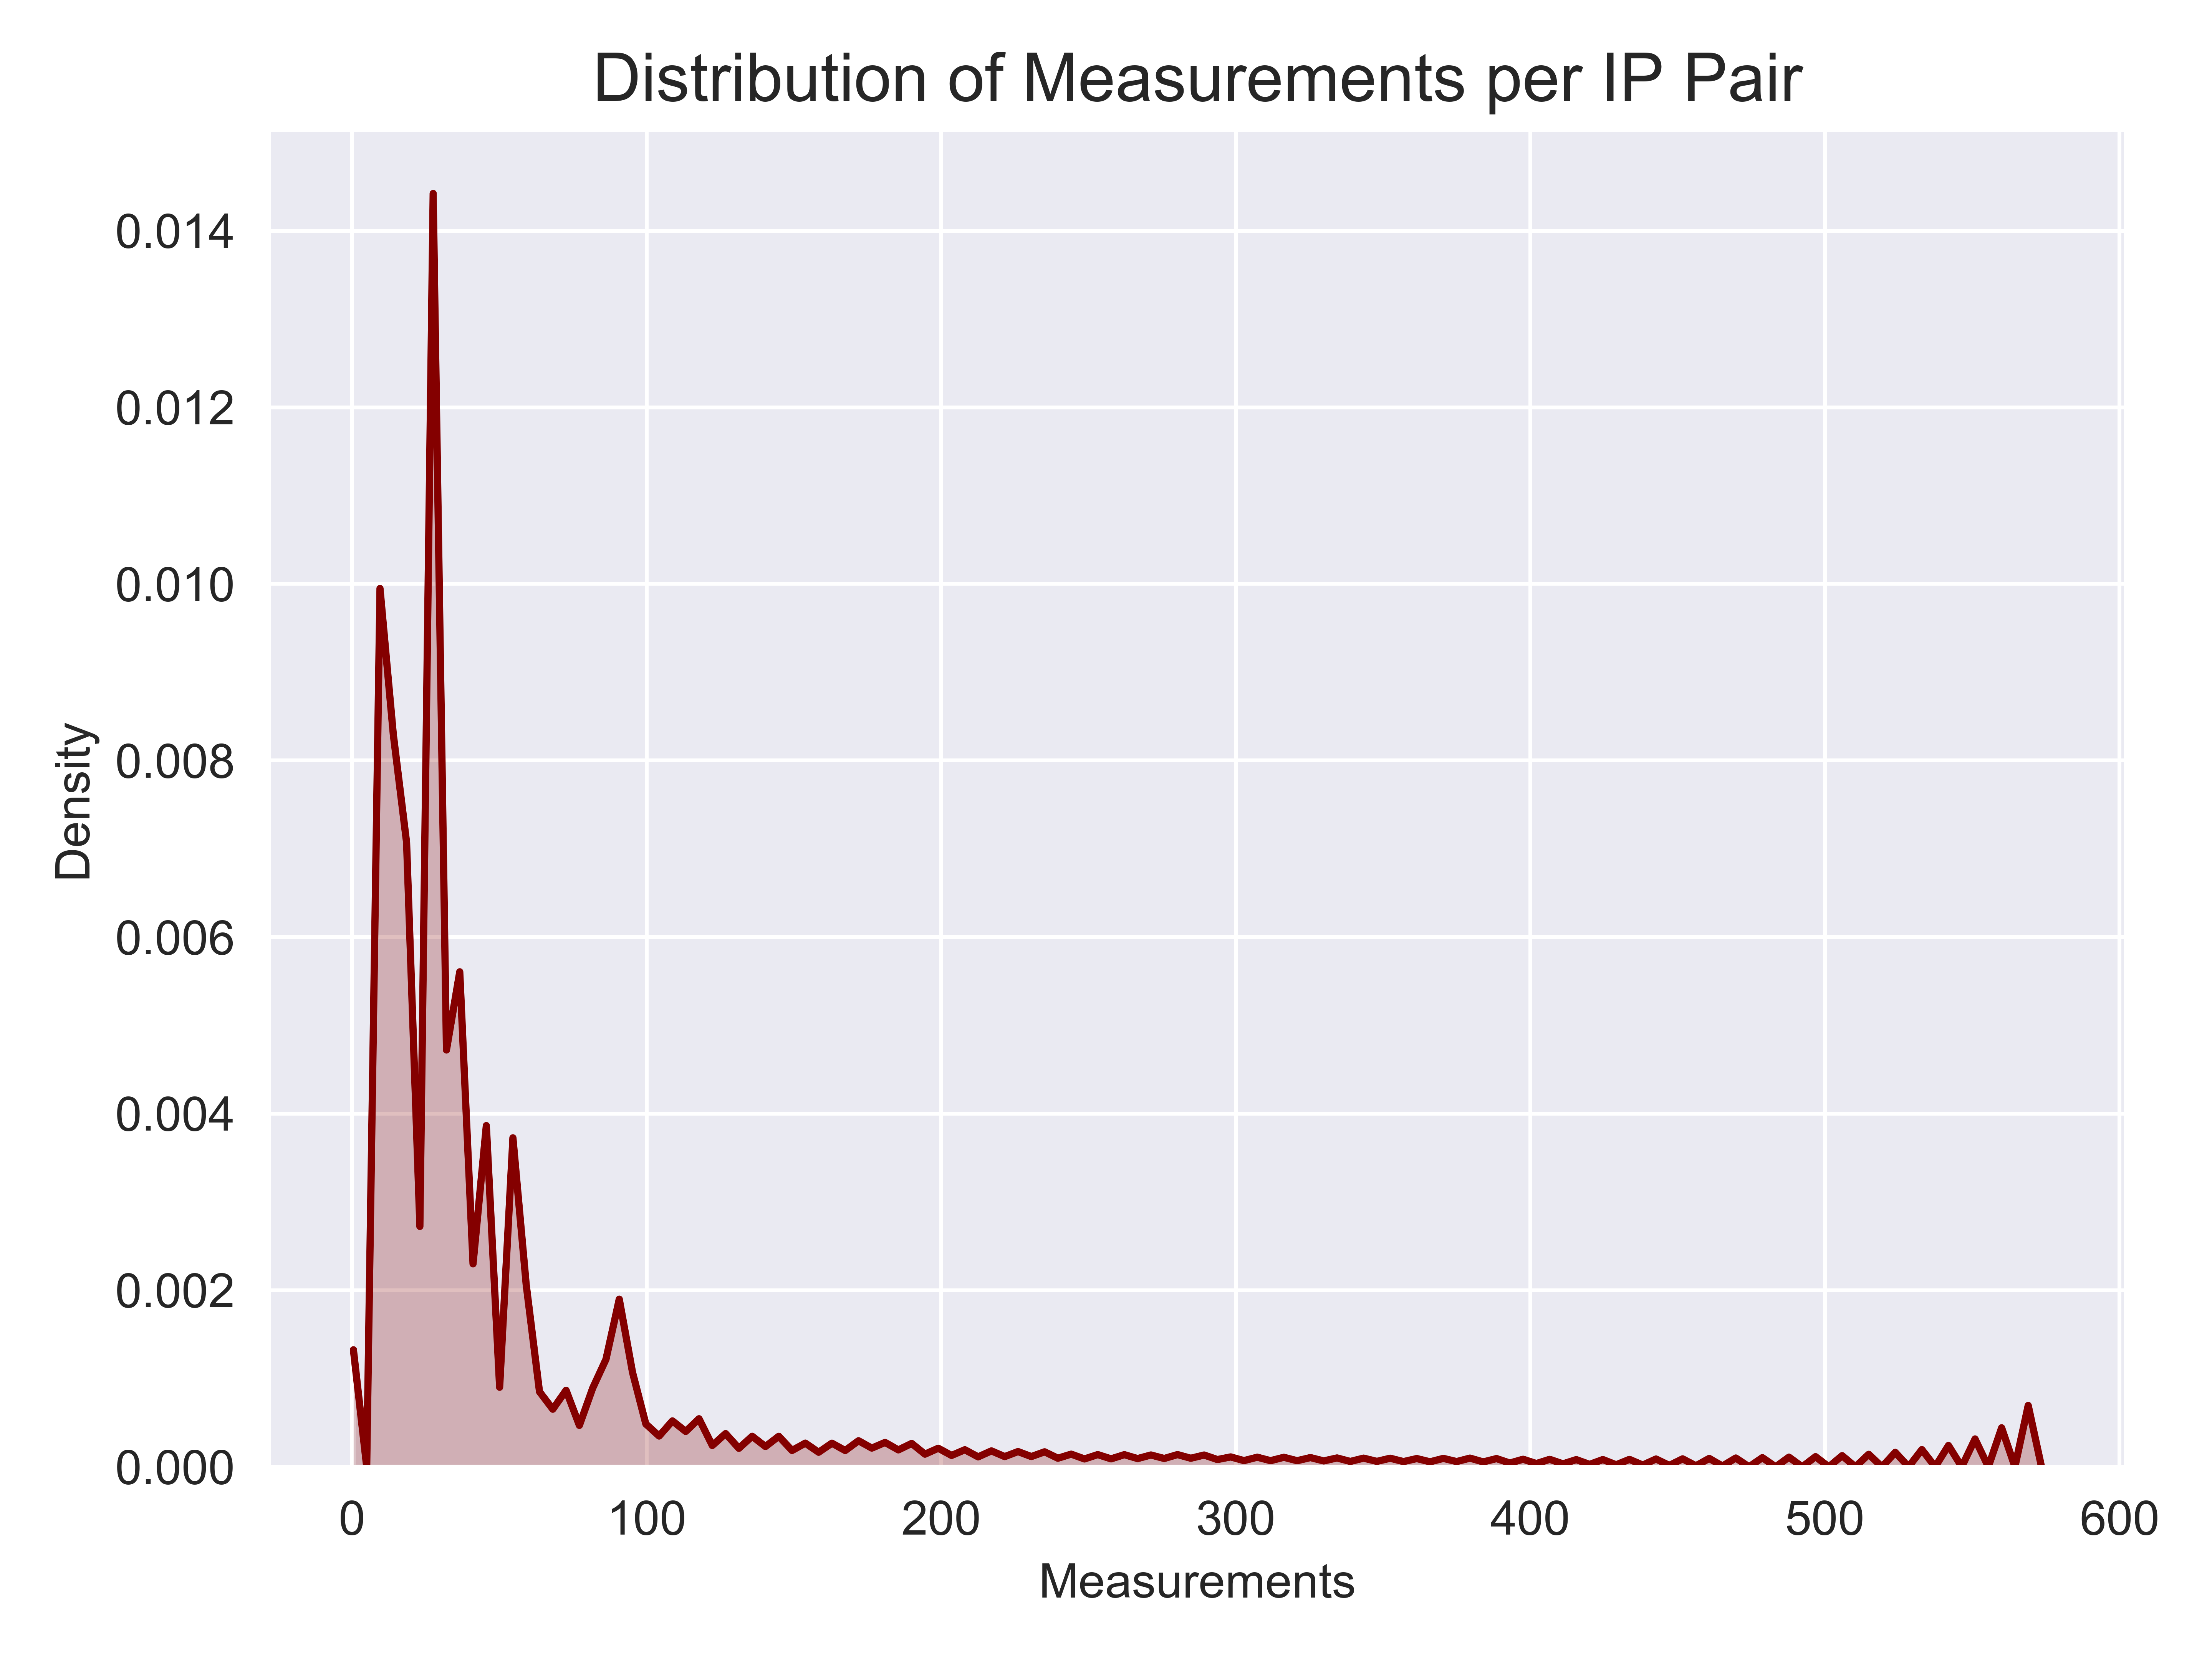
\includegraphics[width=0.75\textwidth]{caida/measurements_distribution.png}
    \caption{Distribution of measurements count for each IP pair}
    \label{fig:caida_measurements_distribution}
\end{figure}

\begin{figure}[H]
    \centering
    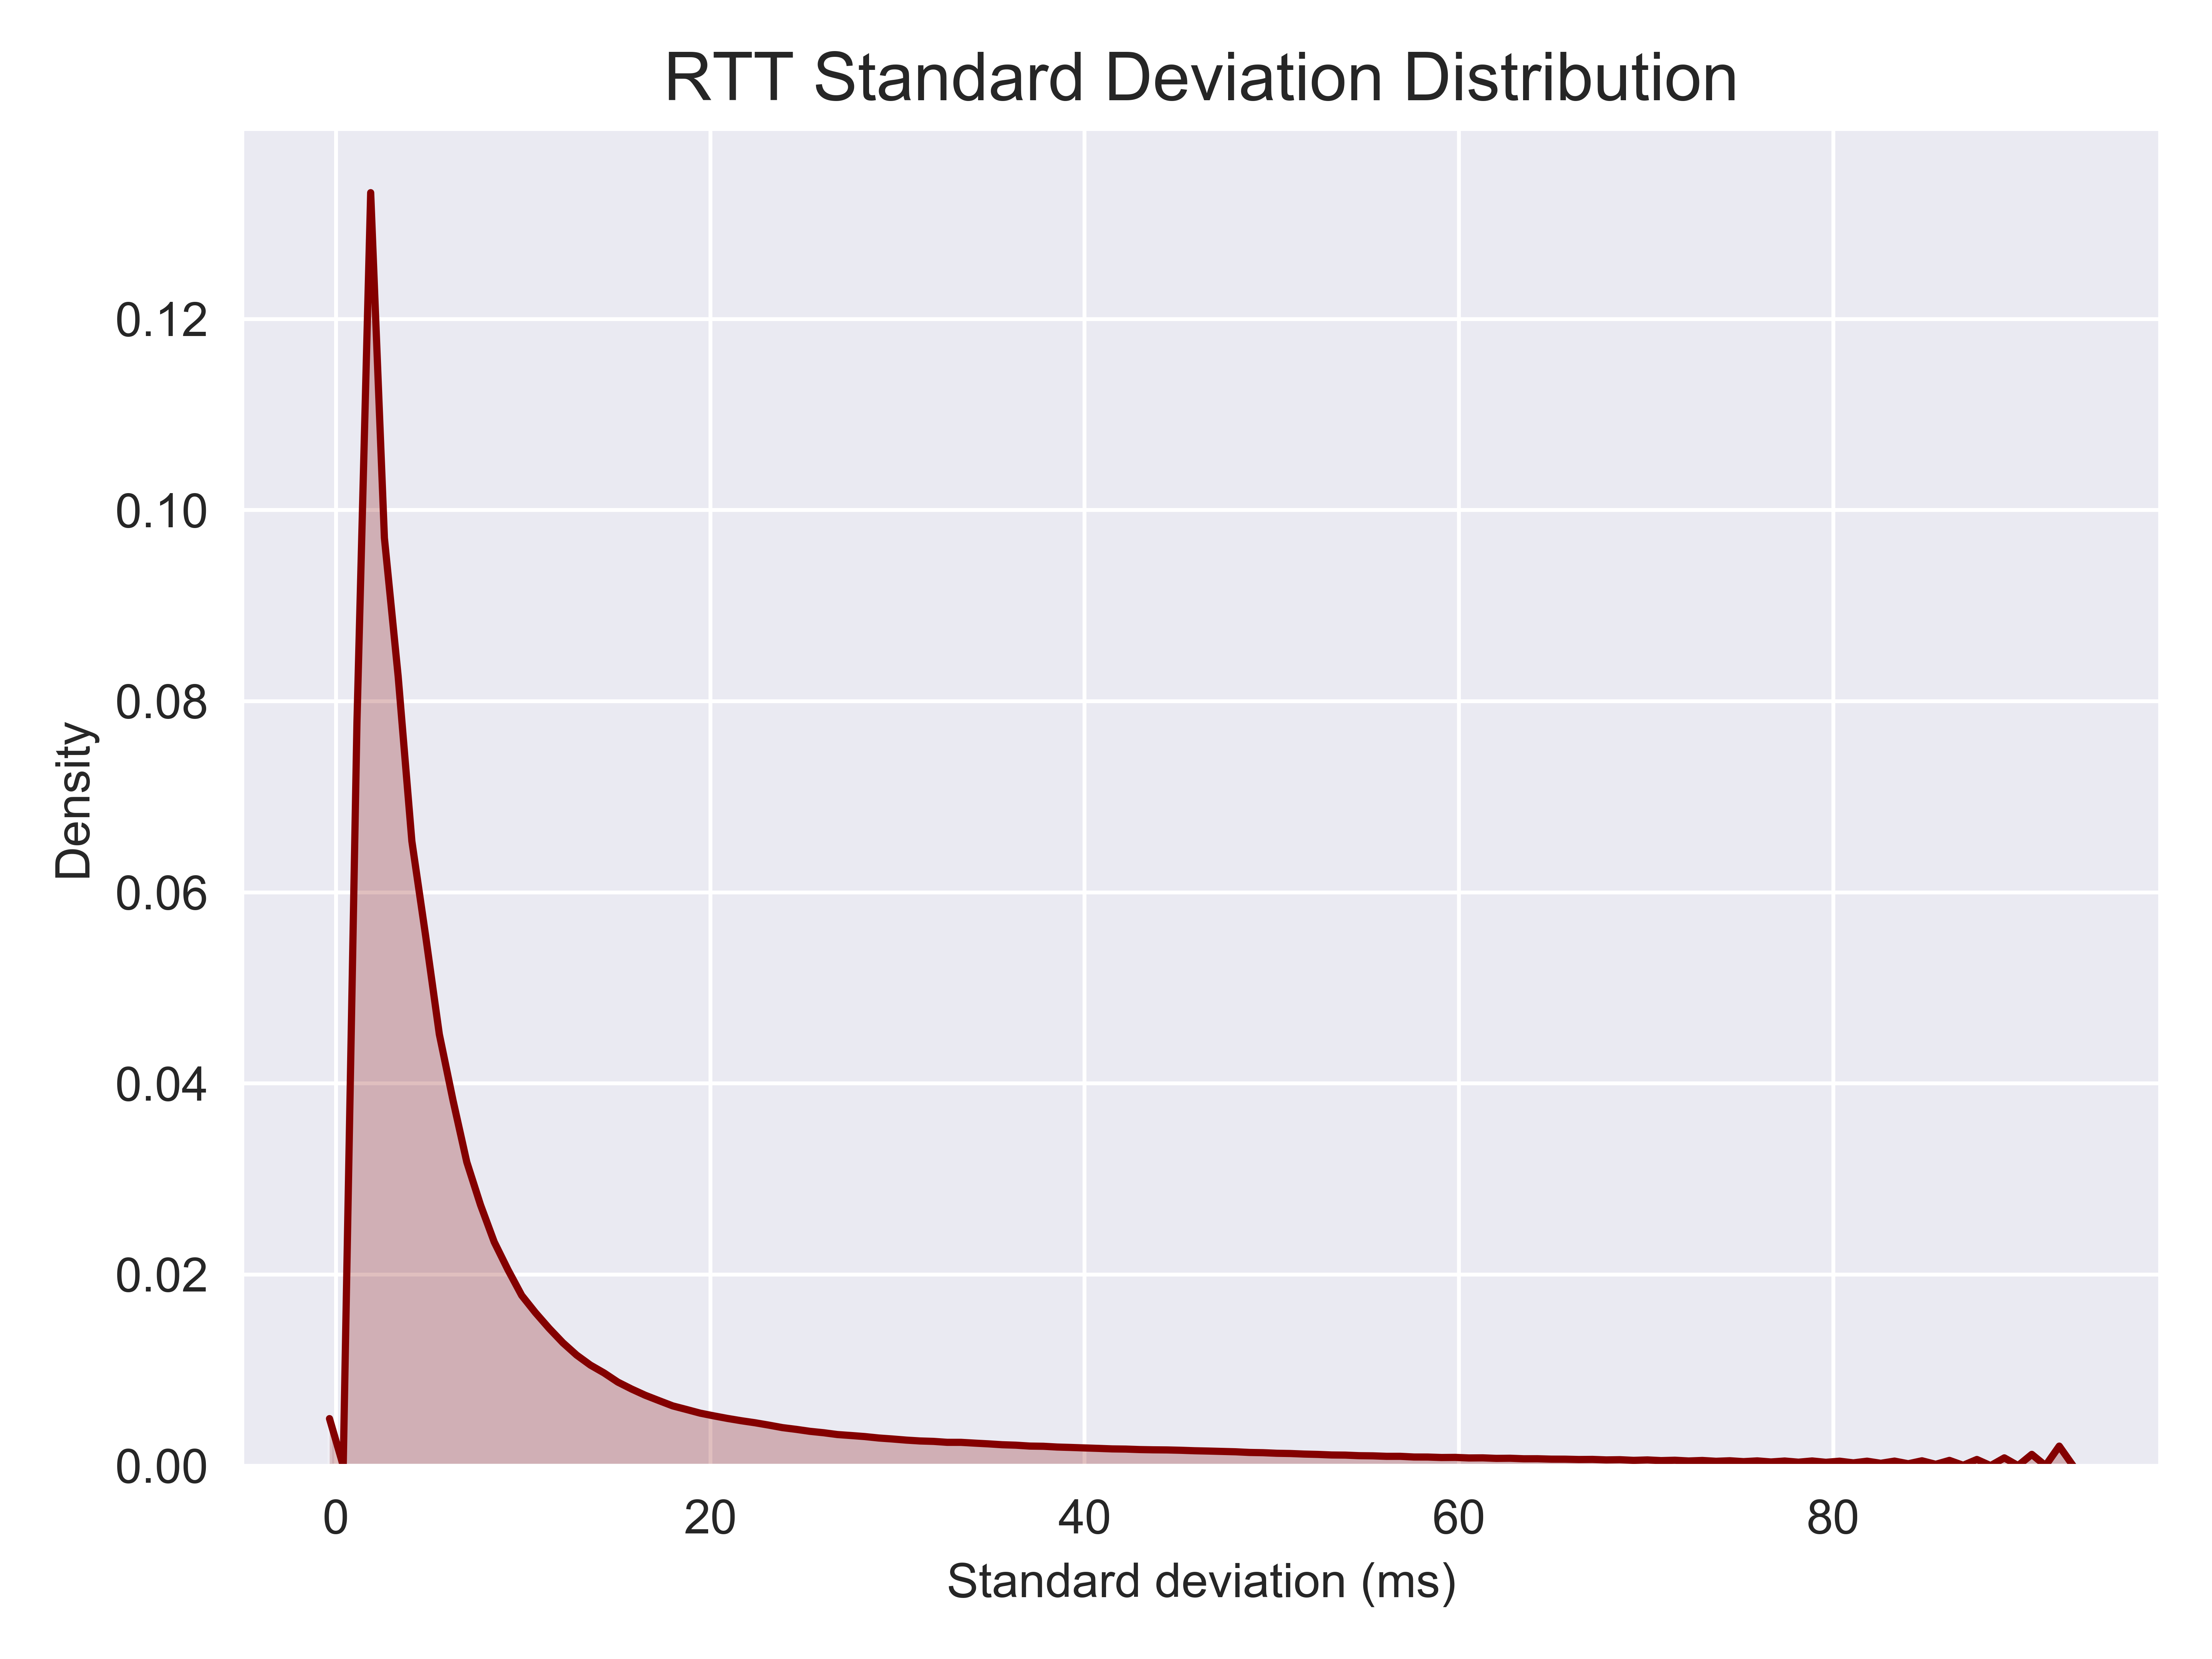
\includegraphics[width=0.75\textwidth]{caida/rtt_stdev_distribution.png}
    \caption{Distribution of IP pair standard deviations}
    \label{fig:caida_stdev_distribution}
\end{figure}

To assess the quality of the measurements for each \ip pair we first turn to the standard deviation. \autoref{fig:caida_stdev_distribution} shows the distribution of standard deviations across all measured \ip pairs (for charting purposes, pairs with only one measurement were interpreted as 0 standard deviation). The chart shows an incredibly smooth curve in with the overwhelming majority of pairs having standard deviations well below 20 ms. To further improve upon that analysis we next turned to \cvs as a measurement of data quality. \cvs are a dimensionless measure that can be interpreted the same across any data set, where lower means better. \autoref{fig:caida_cv_distribution} shows the distribution of \cvs for all \ip pairs, with the majority of \cvs below 0.1 --- in other words, very good data with low spread.

\begin{figure}[H]
    \centering
    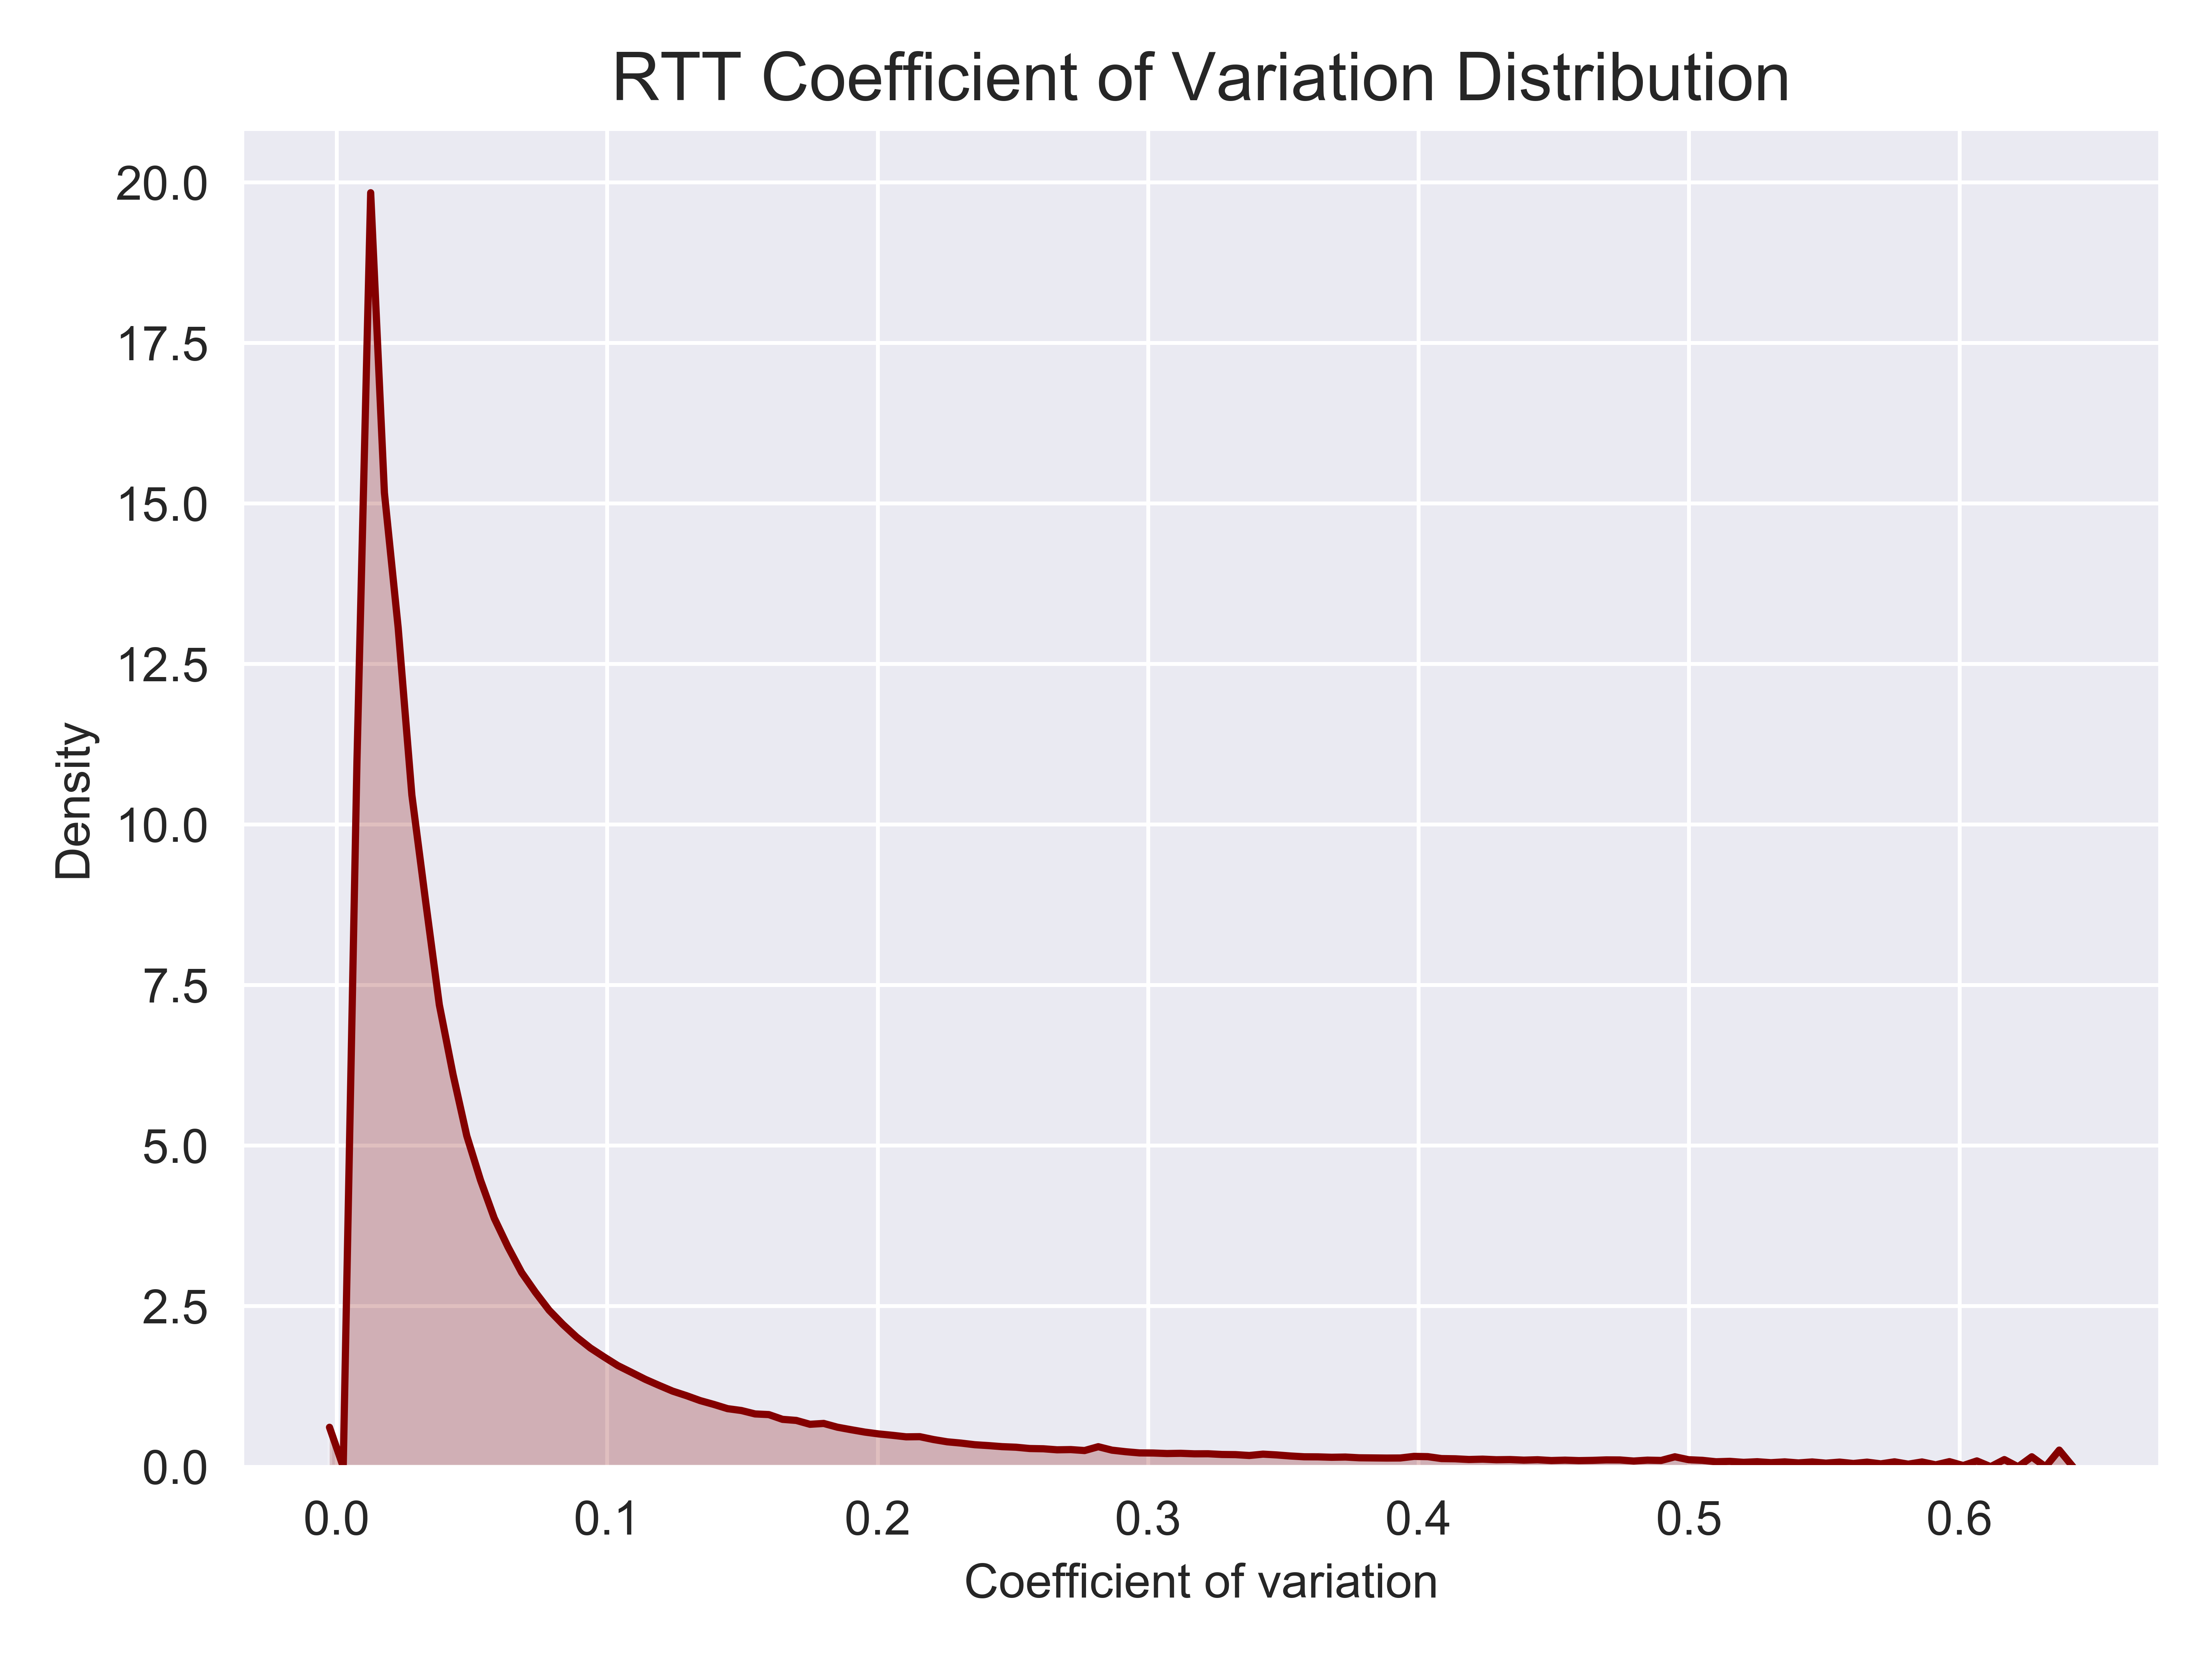
\includegraphics[width=0.75\textwidth]{caida/rtt_cv_distribution.png}
    \caption{Distribution of IP pair coefficients of variation}
    \label{fig:caida_cv_distribution}
\end{figure}

\subsection{Primitive Connectivity Analyses}

Each data point comprises an \ip pair, but each destination \ip --- that is, each \ip that a \caida or \ripe atlas node ran a measurement against --- appears many times, at least once for every node that ran a measurement against it. Averaging these won't work (it makes little sense to average together measurements from a server in Boston with a server in Moscow against a server in New York, since the Moscow measurement node will naturally report a much higher \rtt), so normalization is needed. The first normalization attempted was simple normalization by distance, which returns values in \si{\milli\second\per\kilo\meter} since milliseconds and kilometers are natural units for \rtts and distance, respectively.

\begin{figure}
    \centering
    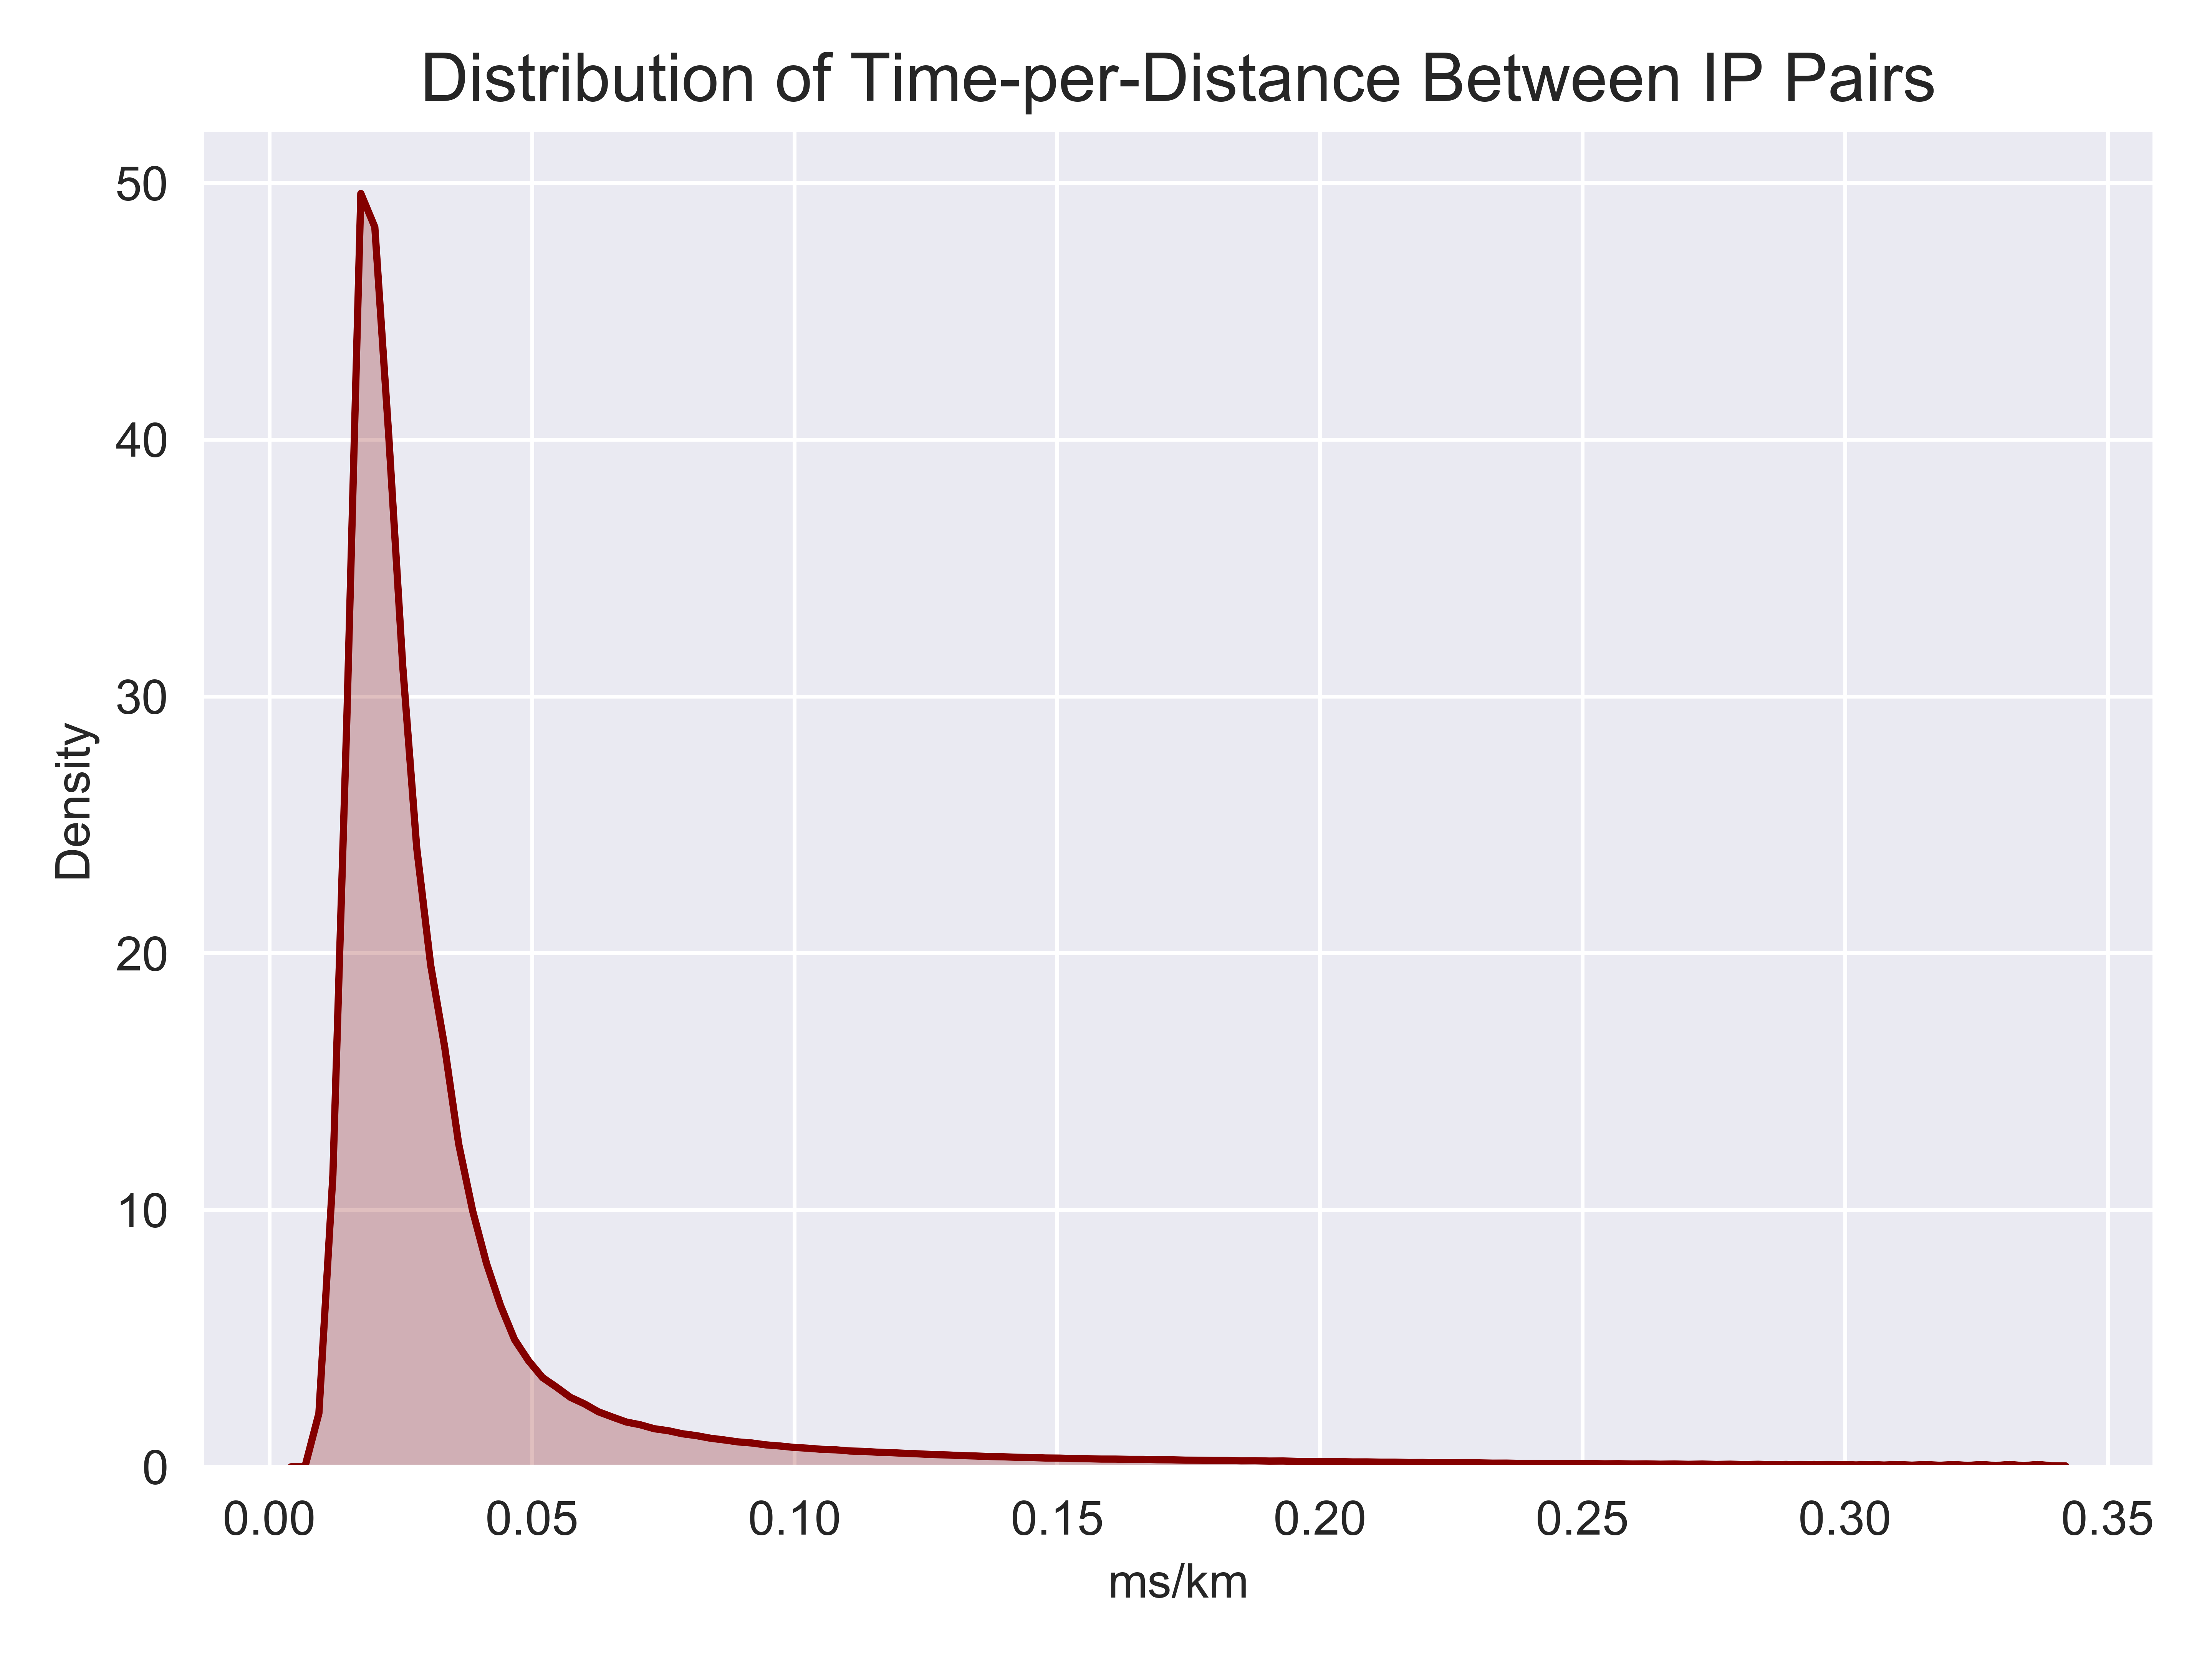
\includegraphics[width=0.75\textwidth]{caida/ms_per_km_distribution.png}
    \caption{Distribution of milliseconds-per-kilometer connectivities}
    \label{fig:caida_ms_per_km_distribution}
\end{figure}

The \si{\milli\second\per\kilo\meter} distribution shown in \autoref{fig:caida_ms_per_km_distribution} is remarkably uninformative on its own, but it does demonstrate an important feature. Normalization succeeds in removing the bimodality of the \rtt distribution shown in \autoref{fig:caida_rtt_distribution} without removing \textit{all} the spread of the data. This both further affirms the earlier hypothesis about the cause of the bimodality and gives cause to believe that geographic charting may yield interesting results.

Unfortunately this metric is challenging to chart with any color scale. The majority of values are between 0.0 and 0.05 \si{\milli\second\per\kilo\meter} but values an order of magnitiude higher must also be charted, and a log scale fails to capture important data. To solve this, a new metric based on efficiency relative to the speed of light was devised.

The speed of light is \SI{299.79246}{\kilo\meter\per\milli\second} (shown in milliseconds and kilometers for ease of distance and relevance to \rtts), so the theoretical minimum \rtt between two points \textapprox 300 km apart is \textapprox2 milliseconds -- one millisecond one way, another on the return trip. All telecommunications happens over electromagnetic mediums, be it fibre optic cables or copper wires, and thus have a transmission delay equal to the speed of light. If the \rtt was higher than 2 milliseconds, there must logically be some loss somewhere in the network, whether that means poor infrastructure or wiring that doesn't follow a straight line to the source -- either way, an inefficiency. The smaller the \rtt, the higher the efficiency, and vice versa. This has the desirable quality that extreme outliers are always between 0 and 1 regardless of how high the \rtt is. The formula for speed-of-light-efficiency based on \rtts is shown in formula \ref{form:speed_of_light_efficiency}.

\begin{formula}[H]
    \begin{equation}
        E = \frac{2d}{t \times 299.79246}
    \end{equation}
    \caption[Formula for speed-of-light efficiency]{Formula for speed-of-light efficiency; $E$ is efficiency as a scalar from 0-1, $d$ is distance in kilometers, and $t$ is the \rtt in milliseconds.}
    \label{form:speed_of_light_efficiency}
\end{formula}

Speed-of-light efficiency can also be thought of as a scalar multiplied by $c$, the speed of light -- it's the equivalent "speed" of a ping. With an improved normalization scheme to work with, subtle differences and patterns can be seen in the data,
as shown in \autoref{fig:speed_of_light_efficiency_distribution}. Also important is that this normalization technique provides with another means of filtering data -- anything above 1.0 efficiency can be removed since it violates the laws of physics by exceeding the speed of light.

\begin{figure}[H]
    \centering
    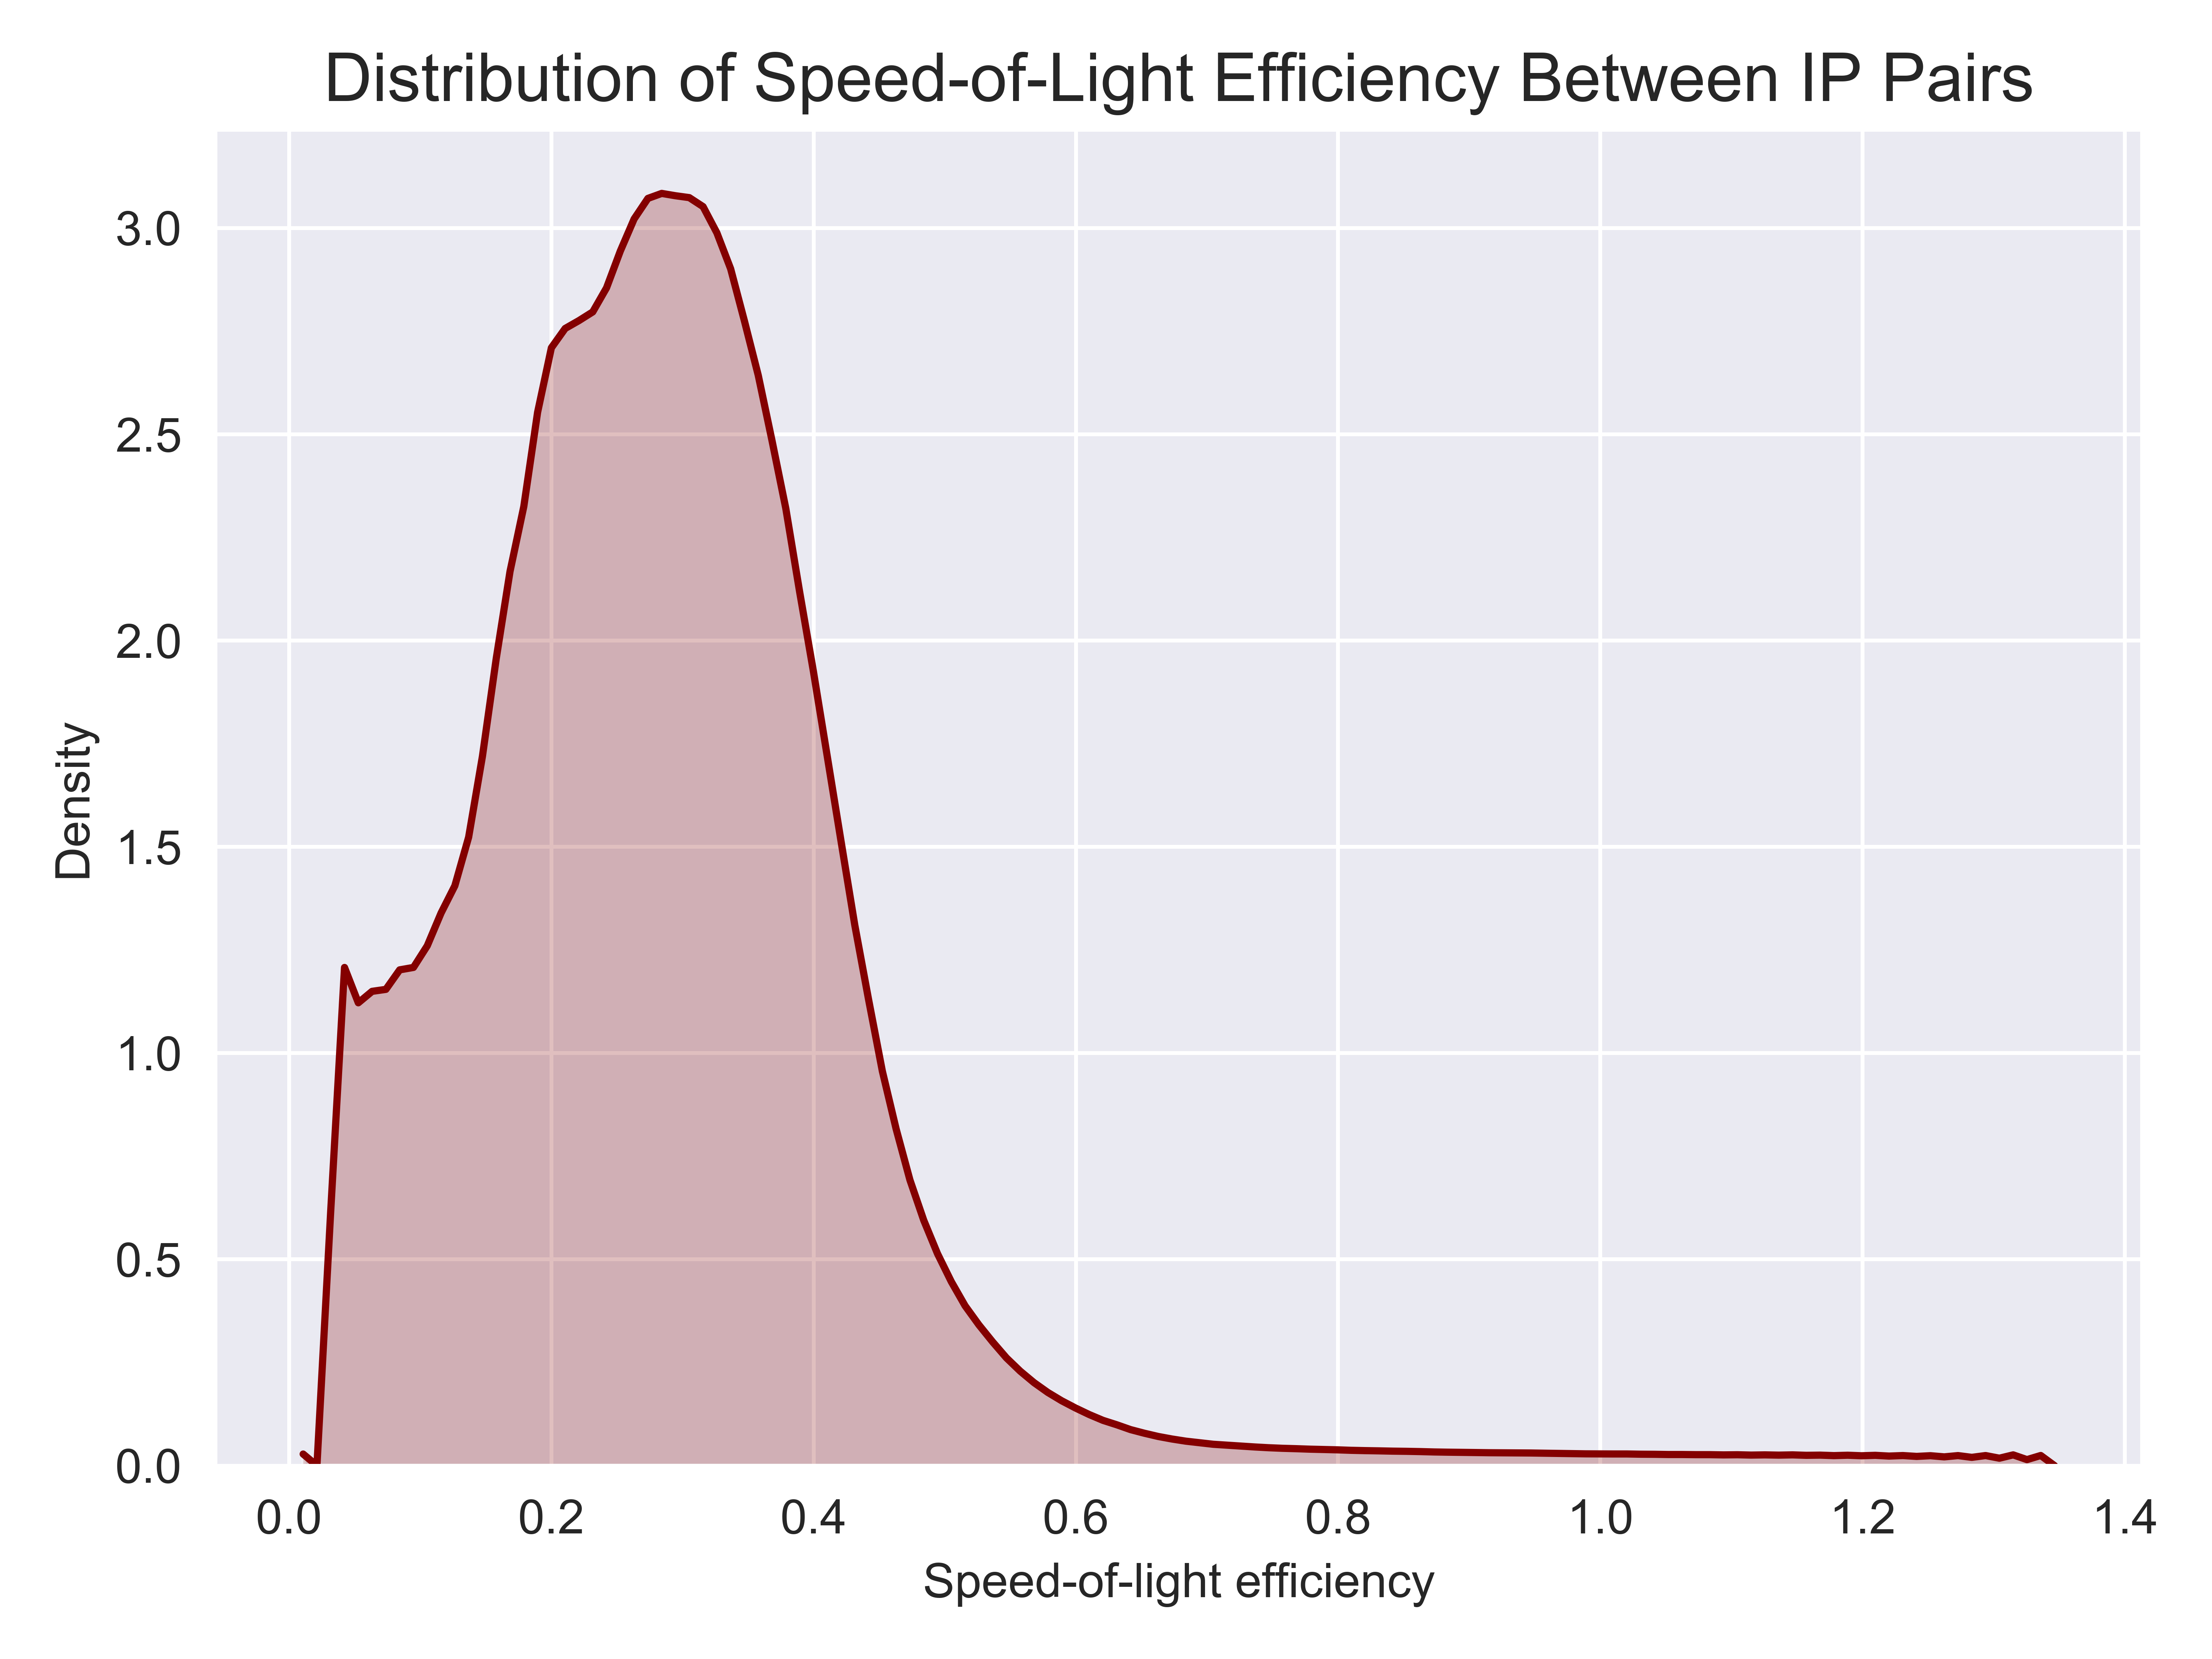
\includegraphics[width=0.75\textwidth]{caida/frac_c_efficiency_distribution.png}
    \caption{Distribution of speed-of-light efficiencies}
    \label{fig:speed_of_light_efficiency_distribution}
\end{figure}

\subsection{Mapping}

The most immediate way of mapping a set of points on a coordinate plane with values attached to each of them is a a simple
scatterplot, but with massive amounts of unevenly distributed data it becomes tough to visualize and draw conclusions. For example, in \autoref{fig:caida_scatterplot} we see point for \textit{every single data point} in the \caida and \ripe Atlas data set that was collected and analyzed.

\begin{figure}[H]
    \centering
    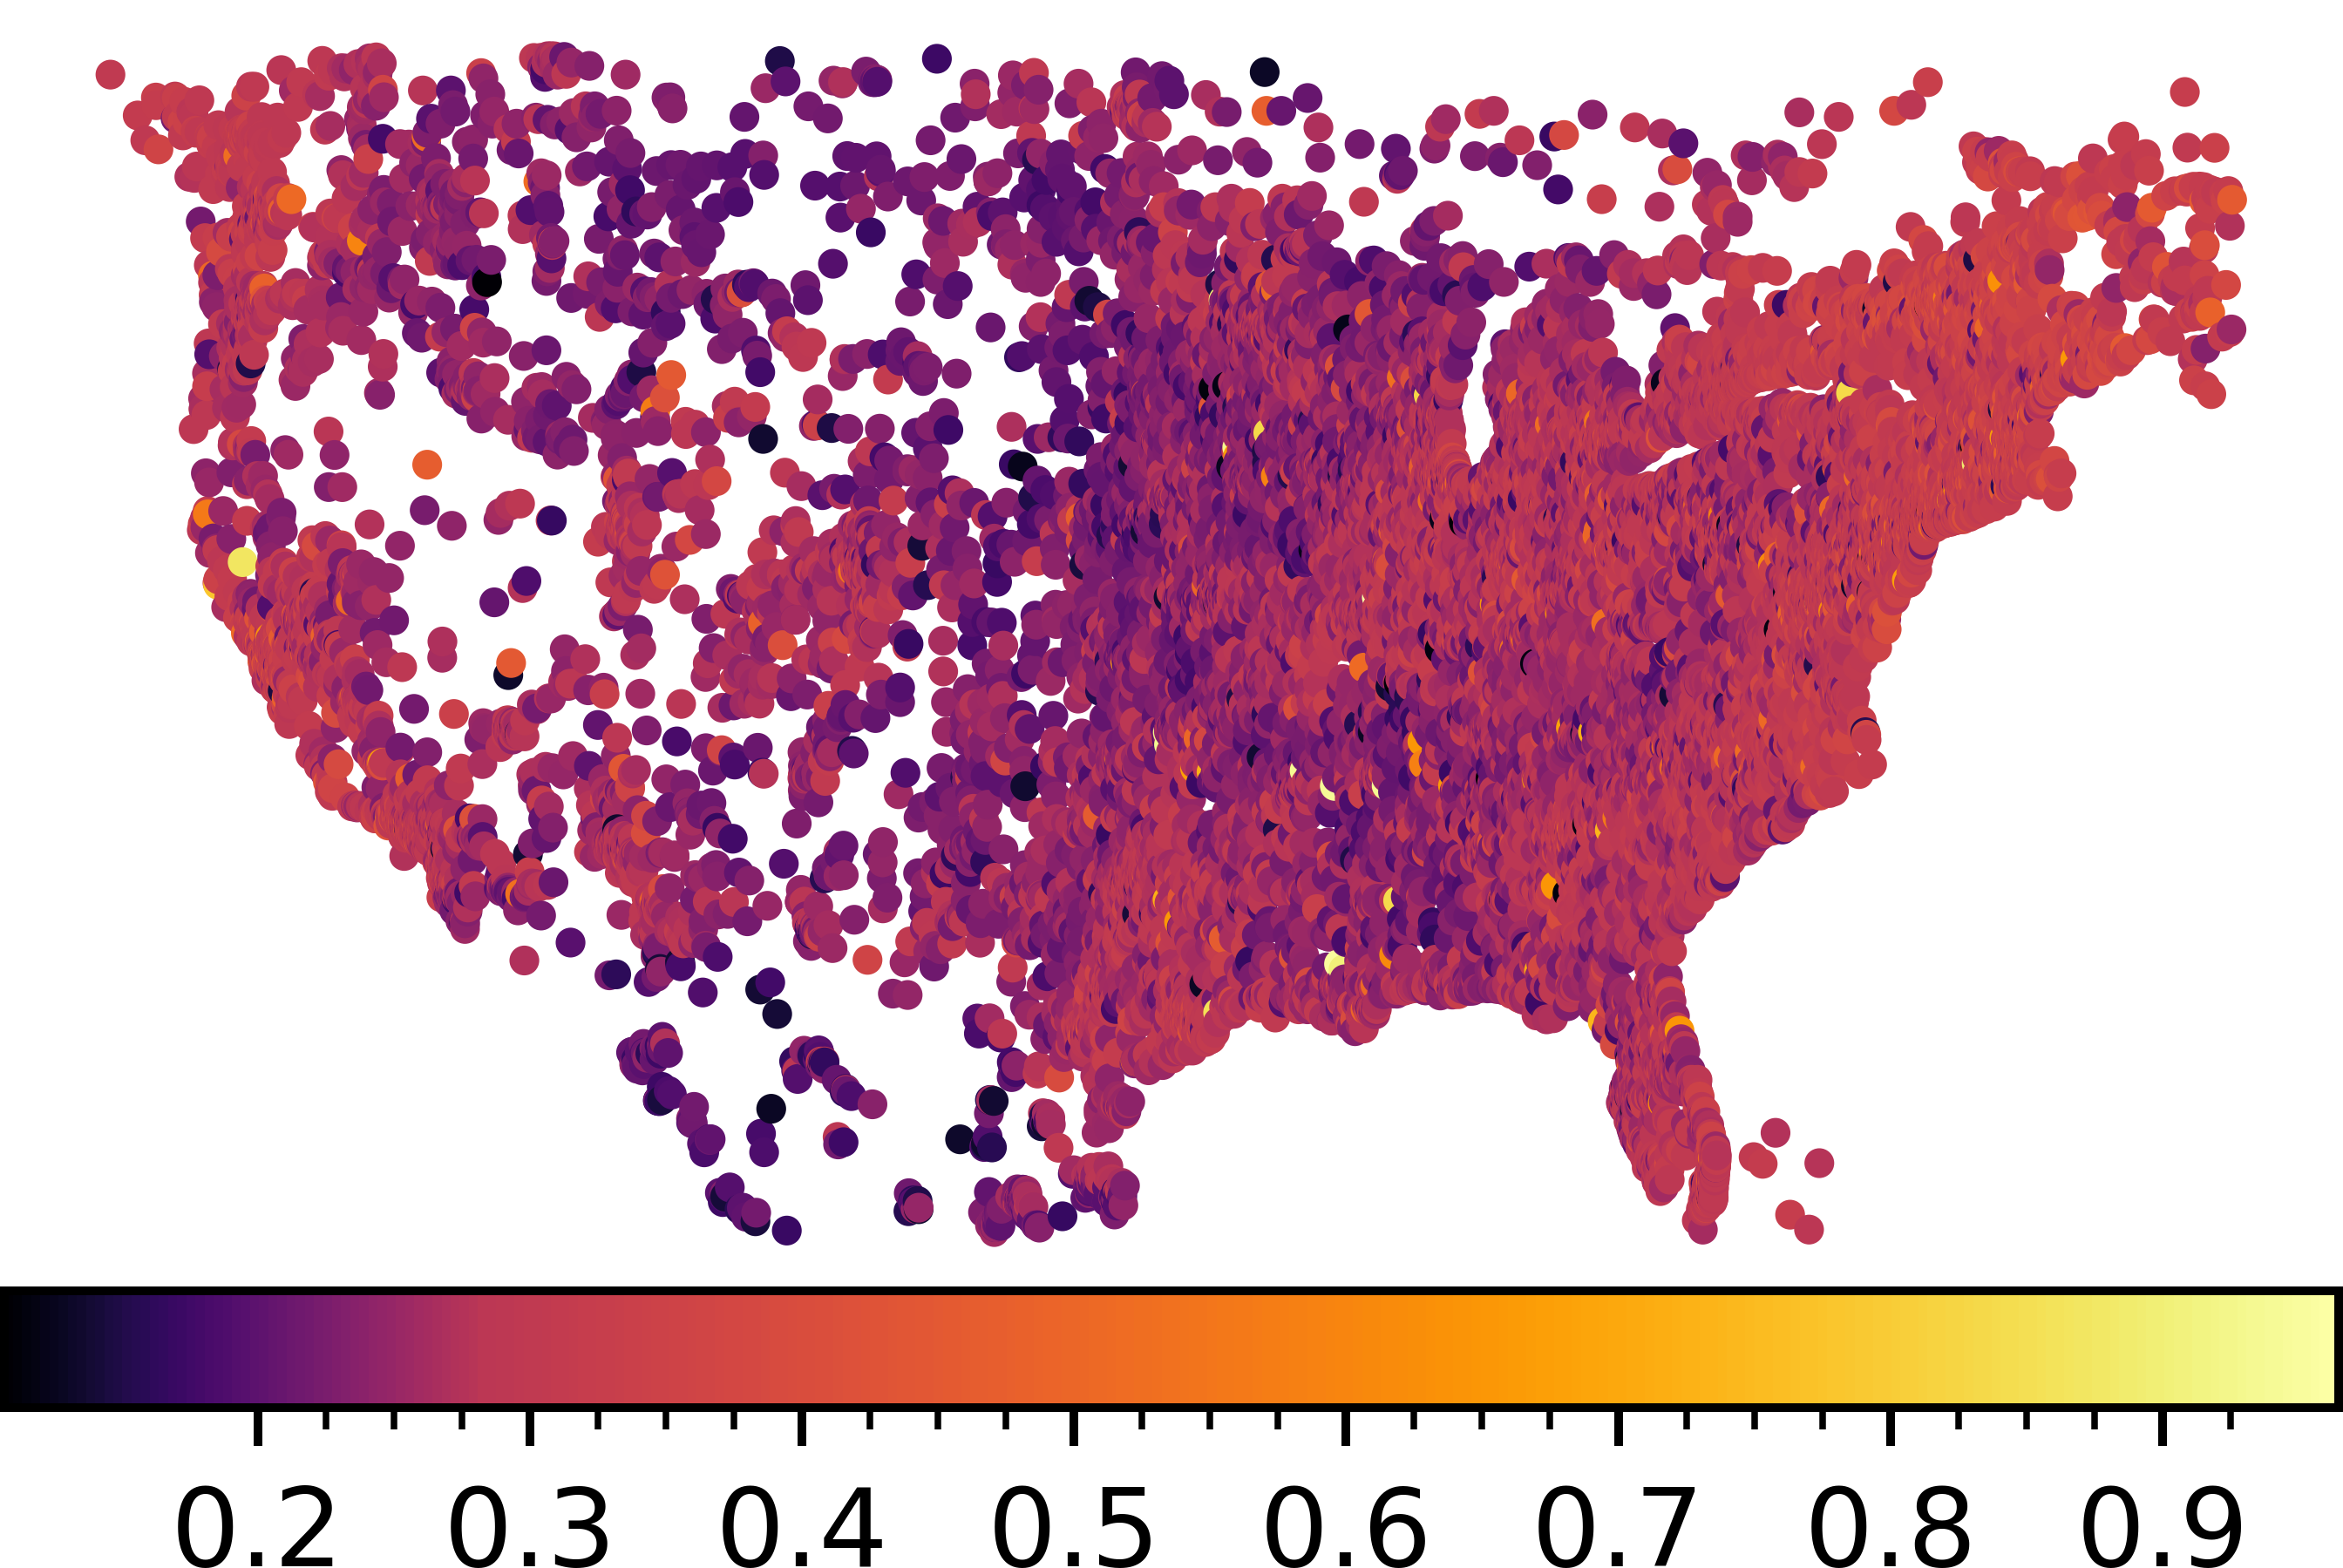
\includegraphics[width=0.75\textwidth]{caida/scatterplot.png}
    \caption{Scatterplot of CAIDA data, normalized and colored by speed of light efficiency}
    \label{fig:caida_scatterplot}
\end{figure}

Some simple relationships can be inferred with moderate difficulty, like better internet connections near the coast or major cities, but otherwise this map is truly only good at confirming that geolocation of IP addresses works. Many areas simply don't have measurements either, and those that appear covered look that way because the dots for each measurement were inflated for visual effect. If they were more accurately represented to-scale as single pixels, the map would be very sparse.

To solve this problem the map needed some interpolation to fill in the gaps and make the data easier to understand. Ideally someone looking at the map should be able to point to a spot on the map and get an estimated value for connectivity at that location, even if there wasn't a measurement at precisely that location. Different methods of interpolation are available, the simplest of which is nearest-neighbor interpolation.

\begin{figure}[H]
    \centering
    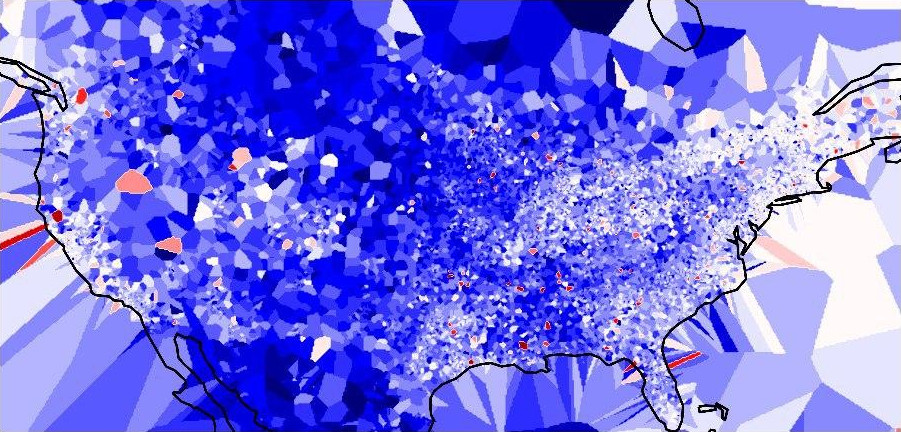
\includegraphics[width=0.75\textwidth]{caida/nearest_neighbor.jpg}
    \caption{Nearest-neighbor (Voronoi) diagram of speed-of-light efficiency data, divergent colormap}
    \label{fig:caida_nearest_neighbor}
\end{figure}

\autoref{fig:caida_nearest_neighbor} shows a nearest-neighbor plot, otherwise known as a Voronoi diagram \cite{Malhotra2017LoveNeighbors}, of the \caida and \ripe Atlas data combined, generated with Python matplotlib and scikit-learn. The colormap is a divergent linear colormap, where blue is worse-than-average and red is better-than-average efficiency. This does an arguably better job of presenting the data, but it's visually noisy and suffers from expanded influence of points in small areas. For instance, consider the large red splotch in Utah, which corresponds to Salt Lake City. While it's likely accurate that the city has far better internet connectivity than its desert surroundings, it is likely inaccurate to say that the areas within the few hundred mile radius shown on the map have the same level of connectivity.

\FloatBarrier

    \section{Cumulative Analysis}\label{sec:results_cumulative}
    
    \newpage
    \chapter{Future work}
    \section{Improving site ping data collection}

One potential issue with the way we selected the images to load for site ping is that we did not consider where the images were hosted. Most websites utilize a \cdn to serve their content, and most of the image files used for the "ping" were, in fact, located on a \cdn. The ping results are therefore more of a measure of the user's connection to that particular \cdn than to the site as a whole. A revised Site Ping app could measure ping times for one object from each domain a site loads content from and take an average.

\section{More accurate IP Geolocation}

One of the things that could improve the quality of the data collected is more accurate \ip address geolocation. One way this could be done would be the use of more then one IP geolocation service and flag data points where the services do not agree as questionable. Another way geolocation could be improved would be through the use of up to date of a constantly updating database. \ip addresses to move around, even across state lines, based on how the \isp decides to allocate them. Using a continuously updated database would allow for each data point to be logged exactly where it is.

\section{More recursive and authoritative servers for each state}

One of the issues with the \dns cache manipulation method is that it lacked a recursive \dns server in Rhode Island. Additionally, several states had only a single server of a given type. Therefore, future iterations of this method could expand the geographic diversity of servers under test.

\section{Backbone Analysis}

One of the methods discussed in \cref{sec:design_unused_methods} is "backbone analysis". To briefly summarize, the idea was to to examine every indirectly calculated hop (\cref{sec:caida_results}) from the \caida and \ripe atlas dataset and consider those as edges on a graph, where the endpoints of the hop are vertices on the graph. A \textit{massive} graph could be established in this way, giving rise to numerous possibilities for analysis based in graph theory.

Using graph theory methods it would be possible to identify nodes that are part of the internet backbone, and measure connectivity to \textit{those} instead. This provides a far more centralized region of the internet to measure connectivity to, which may improve the quality of the analyses if implemented. It would also give insight on what fraction of traffic passes through the backbone, which could be another interesting metric for connectivity.

\section{Surveys \& Subjective User Experience}

Although described in \cref{sec:background}, we ultimately did not pursue methods of collecting data on consumer-oriented statistics like cost, advertised speeds, data caps, or connection stability. These are harder to gather data on using purely technical means -- there is no series of servers we can query like in the \dns method, and there are no databanks of this sort of information available for scraping. To gather real data on the subject it would be necessary to communicate with actual users instead of just their browsers.

This implies a survey of some kind, asking users to provide quantitative information like how much they pay for internet, how fast their internet seems to be, or what their data cap is. Although more challenging to analyze, gathering data on qualitative measures like apparent connection stability may also be useful, although less reliable. These are methods that we did not consider at the start of our project, but that future researchers may be interested in pursuing.

\section{IPv6 Availability}

As mentioned in \cref{sec:connectivity_defs} it might be useful to measure the availability of \ipvs by region, along with mitigating measures like \ipvs-over-\ipvf tunnels. \ipvf address exhaustion is becoming more and more urgent, with the \ripe Network Coordination Center recording exhaustion of their pool in Europe on 25 November 2019 \cite{ReseauxIPEuropeensNetworkCoordinationCentre2019a}. As difficulty of obtaining an \ipvf address increases and network infrastructure is strained further, future researchers will likely want to examine \ipvs availability as a metric for whether internet connections will even be possible in a region.

    
    \chapter{Conclusion}
    1. DC Best
2. Coasts are good
3. Montana bad
4. In between? Can't really say
5. Alaska does not exist
6. Wyoming, what the fuck? 

    
    % TODO Make sure appendix formatting works correctly
    \begin{appendices}
        \chapter{Github Repositories}\label{sec:github-repos}

\Cref{tab:github_repo_table} is a list of repositories created for this MQP, available at:

\url{https://github.com/Internet-Connectivity-MQP-2019}.

\begin{table}[h]
    \centering
    \small
    \begin{tabular}{p{0.35\linewidth}|p{0.55\linewidth}}
         Name & Purpose \\
         \hline
         
         data & Collection of datasets for this project. \\
         
         DigForPy & Python wrapper for the \texttt{dig} utility. Used by DNS\_Testing and Website Resolution.\\
         
         DNS\_Analytics & Scripts used to analyze the \dns cache manipulation data. \\
         
         DNS\_Testing & Scripts for collecting \dns cache manipulation data. \\
         
         fp & Precursor project for SitePing. Created for CS4241 Webware. \\
         
         JavaScript-Ping-Prototype & Proof of concept code for the Site Ping methodology. \\
         
         MTurkValidator & Python script used to validate Mechanical Turk submissions. \\
         
         SitePing & Collection site for the Site Ping method. \\
         
         SitePingDataAnalysis & Data analysis scripts for the Site Ping data. \\
         
         small-file-finder & Chrome extension to find small objects for use in the Site ping method. \\
         
         tracerouter & Proof of concept code for constantly running traceroutes on a phone for the  road trip concept. \\
         
         traceroute-hopper-cpp & Traceroute hopper, ported from Python to C++ for better performance. \\
         
         traceroute-processing-scripts & Traceroute analysis \& processing scripts for CAIDA, RIPE Atlas, and more. \\
         
         WebsiteResolution & Tool for using the list of recursive \dns servers to determine where websites resolve to from across the country. \\
    \end{tabular}
    \caption{List of Github Repositories}
    \label{tab:github_repo_table}
\end{table}
    \end{appendices}

    %%%%%%%%%%%%%%%%%%%
    %%% BACK MATTER %%%
    %%%%%%%%%%%%%%%%%%%
    
    \backmatter
    
    % It's simpler to disable automatic sectioning for the glossaries and references than it is to fix a bug
    % in table-of-authorship handling. I'm so, so sorry.
    \let\endsection\chapter
    \renewcommand{\section}[2]{}%
    
    % List of acronyms
    % \footnotesize
    \newpage
    \setglossarystyle{mcolindex} % See https://www.dickimaw-books.com/gallery/glossaries-styles/ for styles
    \printglossary[type=\acronymtype]
    \addcontentsline{toc}{chapter}{Acronyms}
    
    \setglossarystyle{index}
    \addcontentsline{toc}{chapter}{Glossary}
    \printglossary
    
    % Bibliography, automagically managed in IEEE style.
    \newpage
    \printbibliography
\end{document}